%%%%%%%%%%%%%%%%%%%%%%%%%%%%%%%%%%%%%%%%%%%%%%%%%%%%%%%%%%%%%%%%%%%%%%%
%      Paper A
%%%%%%%%%%%%%%%%%%%%%%%%%%%%%%%%%%%%%%%%%%%%%%%%%%%%%%%%%%%%%%%%%%%%%%%
\section{Paper A}
\section*{Finite Element solution of the fiber/matrix interface crack problem: convergence properties and mode mixity of the Virtual Crack Closure Technique}

The analysis of bi-material interface cracks, such as the fiber/matrix interface crack or debond, in the context of Linear Elastic Fracture Mechanics hides some peculiar complexities due to the nature of the solution at the crack tip. The solution to the fiber/matrix interface crack problem can be classified into two different regimes~\cite{Paris1996,Varna1997a}: the \emph{open crack} and \emph{closed crack} solution. The distinction between the two lies in the existence of a region of contact between crack faces (contact zone) at the crack tip: if it exists, we talk about a \emph{closed crack} solution, otherwise of an \emph{open crack} solution.\\
The \emph{open crack} solution to the straight bi-material interface crack problem was first proposed by Williams~\cite{Williams1959}, who found the existence of an oscillatory singularity in the stress field at the crack tip of the form

\begin{equation}\label{chap3:paperA:eq:singularitywilliams}
r^{-\frac{1}{2}}\sin\left(\varepsilon\log r\right)\quad\text{with}\quad\varepsilon=\frac{1}{2\pi}\log\left(\frac{1-\beta}{1+\beta}\right),
\end{equation}

in both Mode I and Mode II. In Eq.~\ref{chap3:paperA:eq:singularitywilliams}, $\beta$ is one of the two parameters introduced by Dundurs~\cite{Dundurs1969} to characterize bi-material interfaces:

\begin{equation}\label{chap3:paperA:eq:dundursbeta}
\beta=\frac{\mu_{2}\left(\kappa_{1}-1\right)-\mu_{1}\left(\kappa_{2}-1\right)}{\mu_{2}\left(\kappa_{1}+1\right)+\mu_{1}\left(\kappa_{2}+1\right)}
\end{equation}

where $\kappa=3-4\nu$ in plane strain and $\kappa=\frac{3-4\nu}{1+\nu}$ in plane stress, $\mu$ is the shear modulus, $\nu$ Poisson's coefficient, and indexes $1,2$ refer to the two bulk materials joined at the interface. Due to the nature of singular solution at the crack tip in the \emph{open crack} case, the definition of Stress Intensity Factor (SIF) $\lim_{r\rightarrow 0}\sqrt{2\pi r}\sigma$ diverges and is not anymore valid~\cite{Comninou1990}. The mismatch in the value of the elastic properties at the bi-material interface makes the configuration a mixed-mode one, but the Mode mixity problem at the crack tip is ill-posed. For the same reason, Mode I and Mode II Energy Release Rate do not converge. A way to circumvent the problem is to evaluate the ERR over a finite instead of an infinitesimal crack increment, which leads naturally to the application of the Virtual Crack Closure Technique (VCCT)~\cite{Rybicki1977,Krueger2004}.\\
The introduction of a finite crack increment makes the ERR sensitive to the mesh. Several authors have investigated the mesh sensitivity of the VCCT used in conjunction with the Finite Element Method (FEM) in the context of the straight bi-material interface crack~\cite{Krueger2013,Sun1987,Sun1989,Manoharan1990,Raju1988,Agrawal2006,Wang2013} and found that: the total Energy Release Rate $G_{TOT}$ does not depend on the mesh size; for a crack under mixed-mode behavior (\emph{open crack} case), Mode I and Mode II depend on the size of the mesh at the crack tip and do not show convergence. The purpose of this first paper is to analyze the mesh dependency of Energy Release Rate in the case of the fiber/matrix interface crack.

\begin{figure}[!h]
\centering
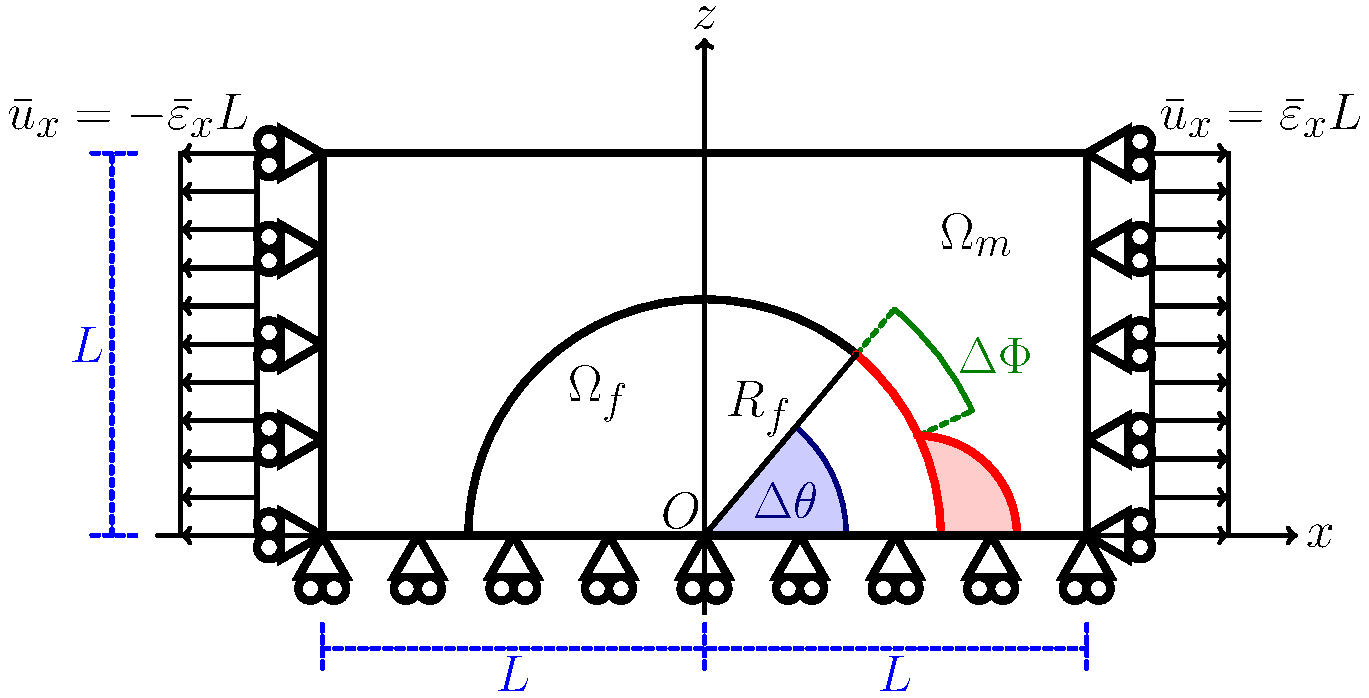
\includegraphics[width=\textwidth]{paperA/RUC.pdf}
\caption{Schematic of the model with its main parameters.}\label{chap3:paperA:fig:modelschem}
\end{figure}

The 1-step VCCT in the force-displacement formulation~\cite{Krueger2004} is considered and applied to the evaluation of the ERR of a debond located on a single fiber placed in a square matrix cell, as shown in Figure~\ref{chap3:paperA:fig:modelschem}. The cell has a size of $2L\times2L$, where

\begin{equation}\label{chap3:paperA:eq:LVf}
L=\frac{R_{f}}{2}\sqrt{\frac{\pi}{V_{f}}},
\end{equation}

$V_{f}$ is the fiber volume fraction and $R_{f}$ is the fiber radius, assumed to be equal to $1\ \mu m$. The occurrence of a contact zone after a critical size of the debond is considered and a contact pair interaction is established between crack faces. The interaction is considered frictionless. As the model is symmetric with respect to the $x$-axis (see Figure~\ref{chap3:paperA:fig:modelschem}), only half of it is explicitly modeled and symmetry conditions are applied to the lower boundary. A constant $x$-strain of $1\%$ is applied to the right and left boundary. Glass fiber and epoxy are considered and their properties are reported in Table~\ref{chap3:paperA:tab:phaseprop}.

\begin{table}[!htbp]
 \centering
 \caption{Summary of the mechanical properties of fiber and matrix. $E$ stands for Young's modulus, $\mu$ for shear modulus and $\nu$ for Poisson's ratio.}
 \begin{tabular}{cccc}
\\
\textbf{Material} & \textbf{$E\left[GPa\right]$}\ & \textbf{$\mu\left[GPa\right]$} & \textbf{$\nu\left[-\right]$} \\
\midrule
Glass fiber    & 70.0  & 29.2   & 0.2  \\
Epoxy    & 3.5    & 1.25   & 0.4
\end{tabular}
\label{chap3:paperA:tab:phaseprop}
\end{table}

The main parameter of the mesh sensitivity study is the angular size $\delta$ of the elements at the crack tip, as shown in Figure~\ref{chap3:paperA:fig:vcctmesh}.

\begin{figure}[!h]
\centering
    \begin{subfigure}[b]{0.8\textwidth}
        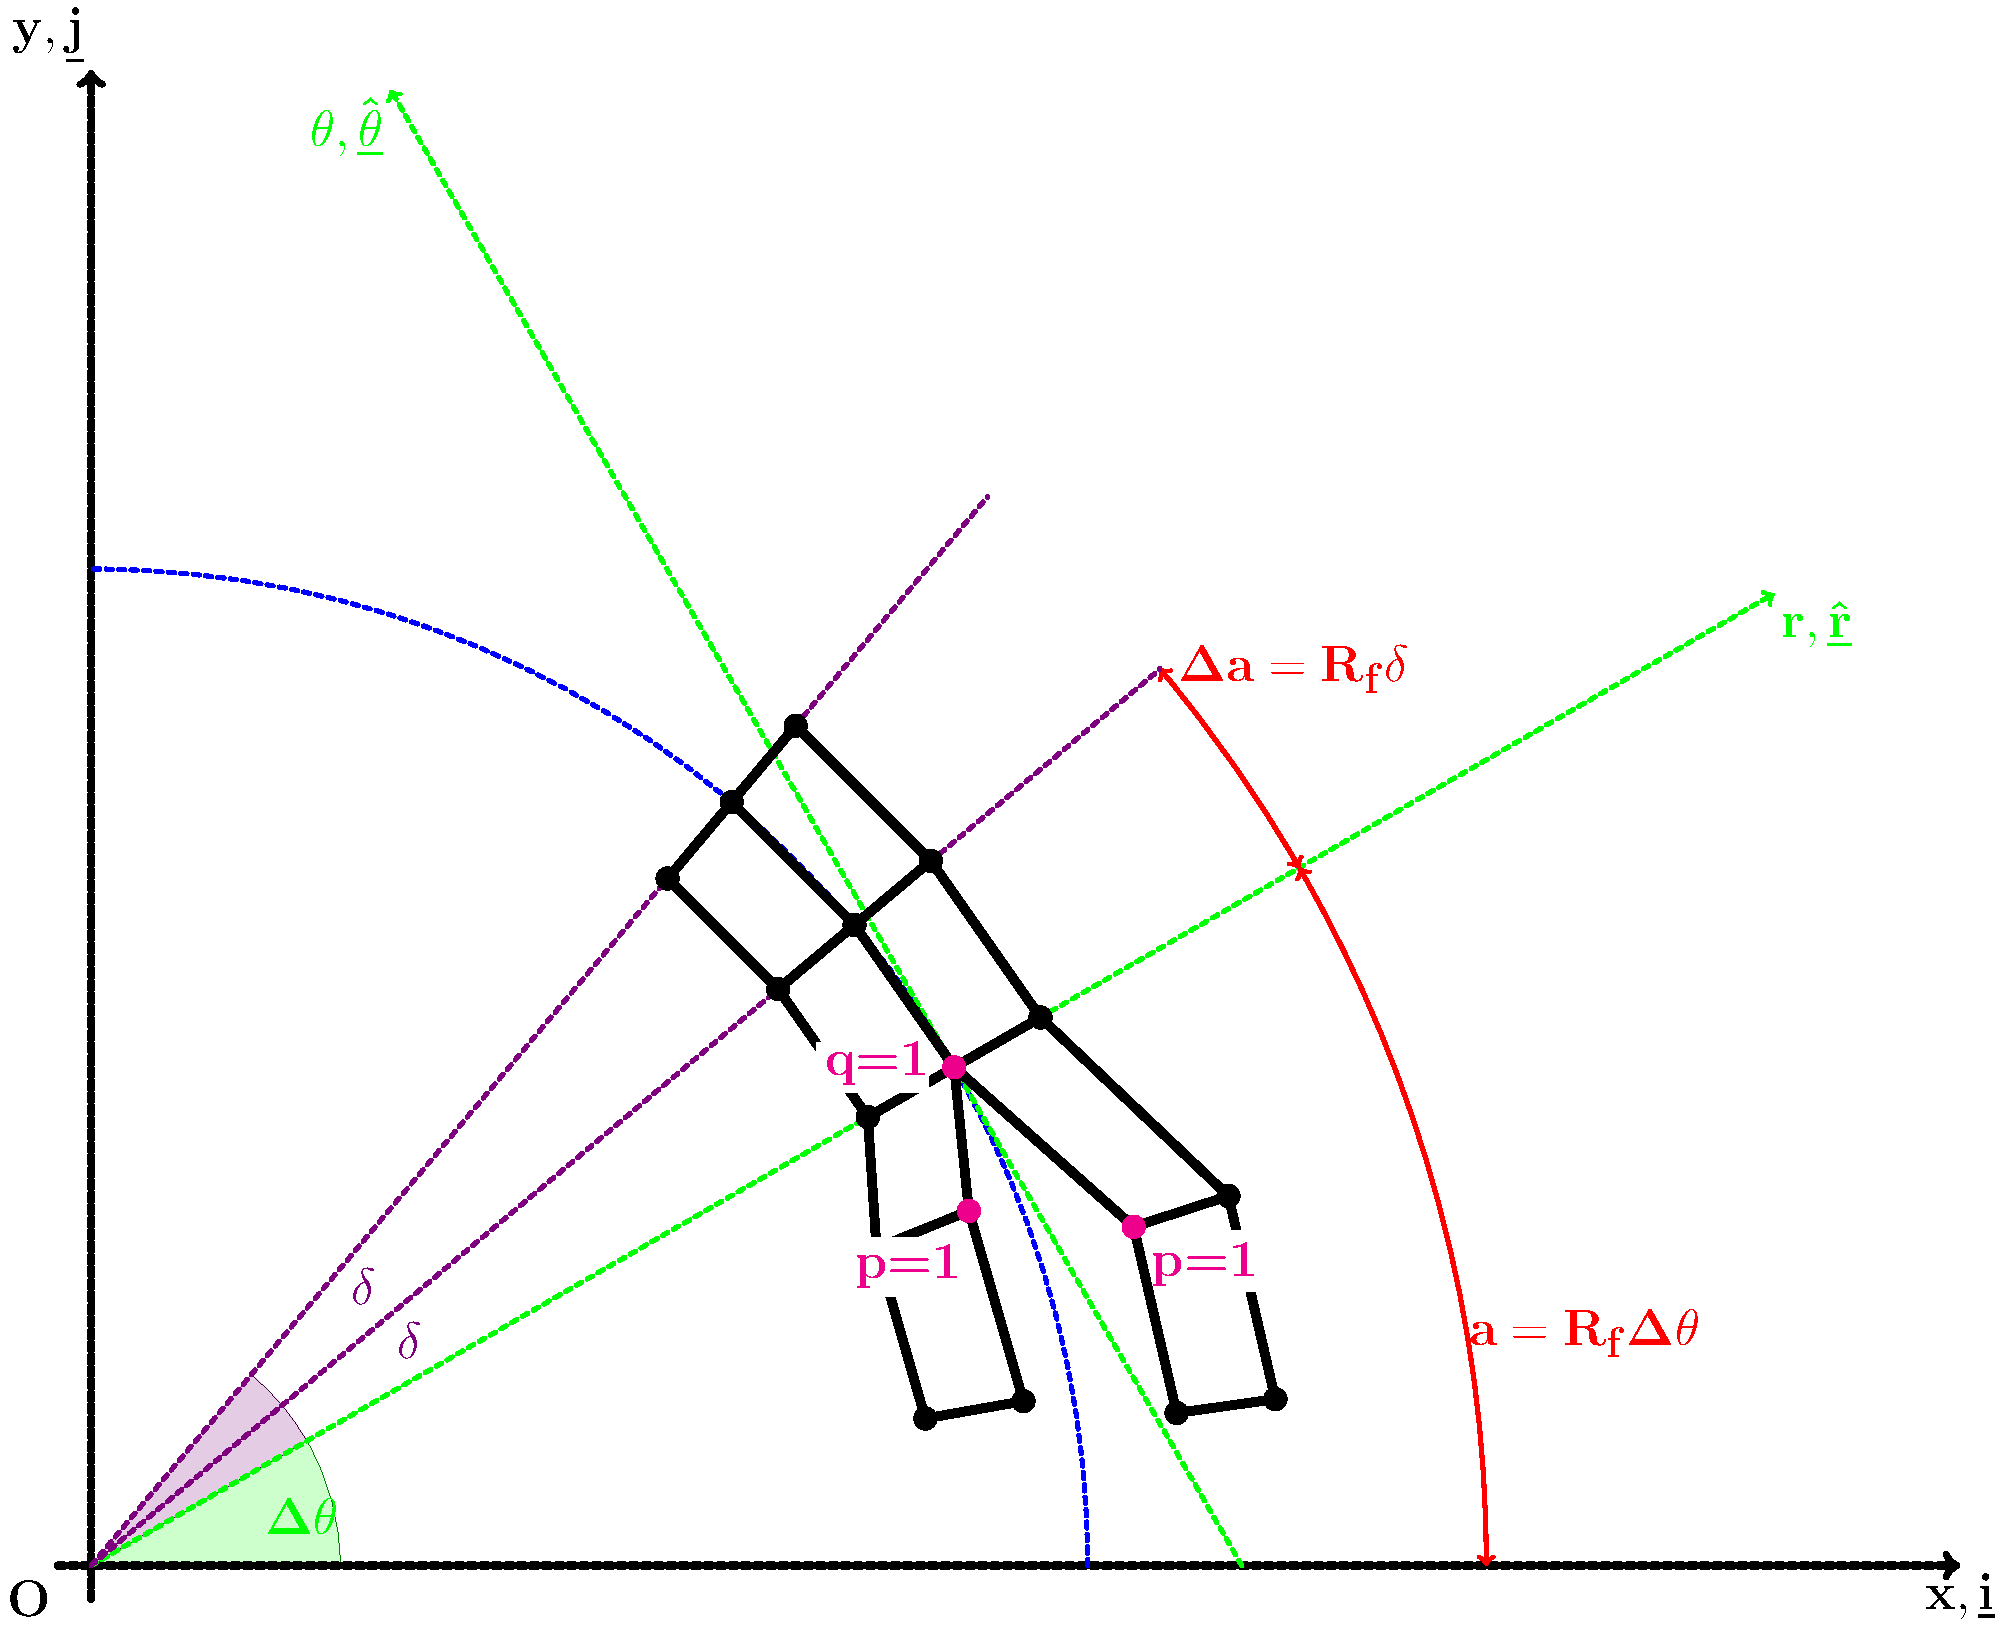
\includegraphics[width=\textwidth]{paperA/VCCT-linear.pdf}
       \caption{\added{Elements with $1^{st}$ order shape functions: $m=1$ and $p,q=1$.}}
    \end{subfigure}

    \begin{subfigure}[b]{0.8\textwidth}
        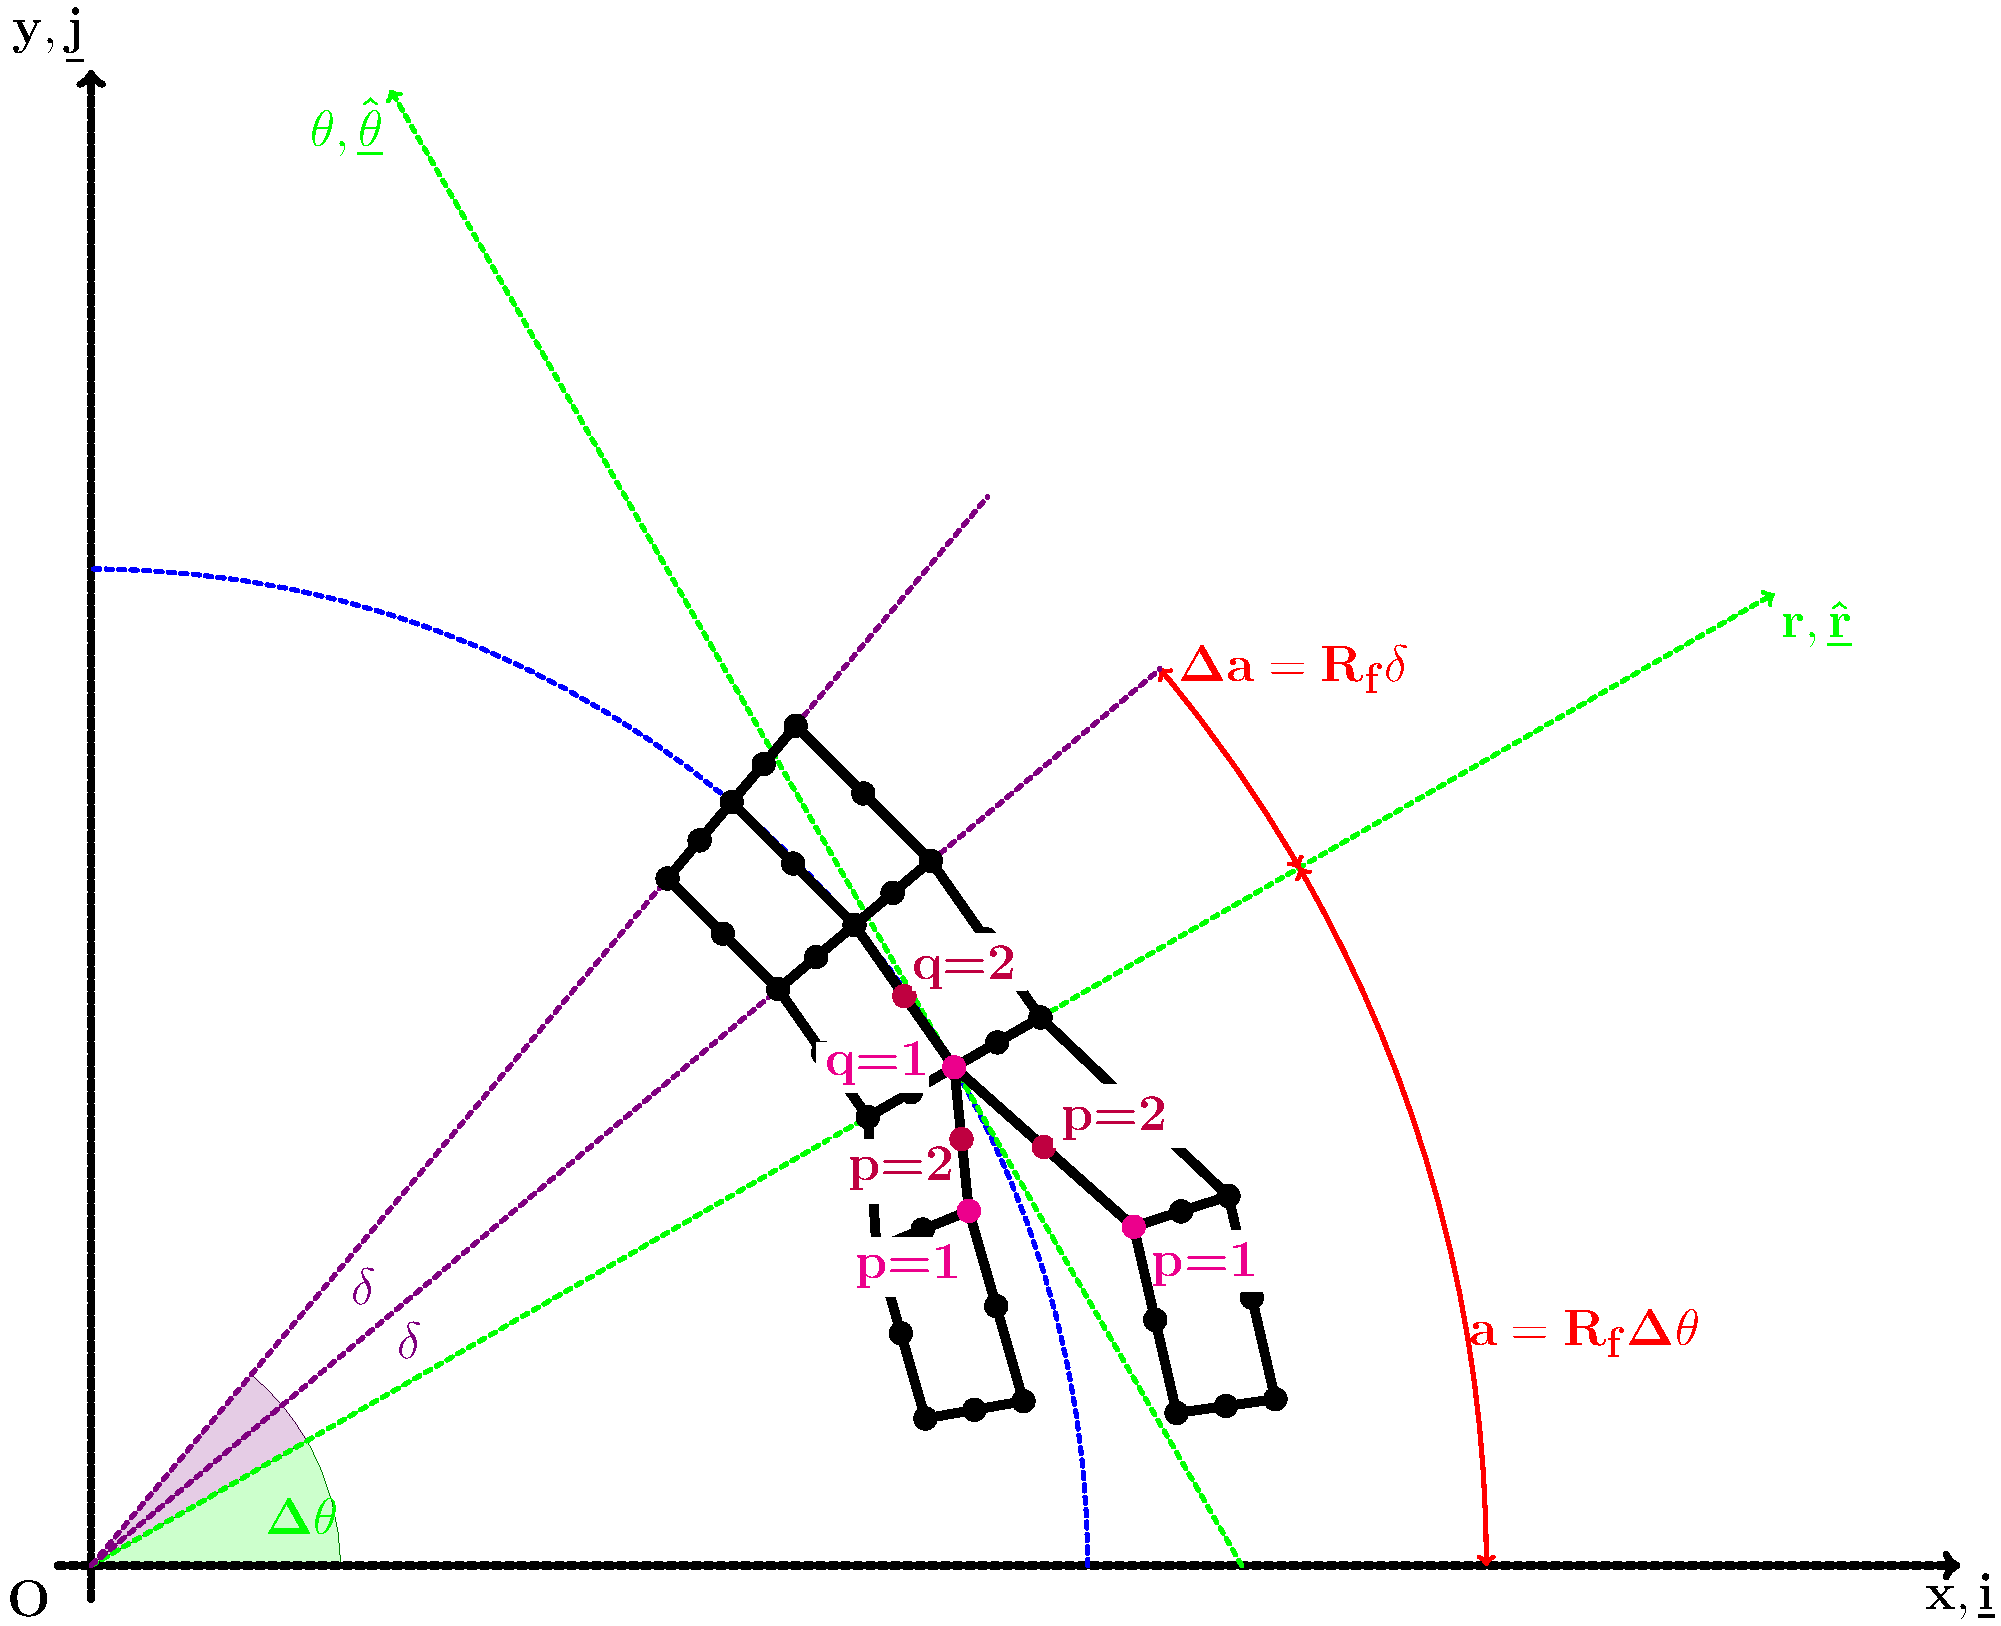
\includegraphics[width=\textwidth]{paperA/VCCT-quadratic.pdf}
       \caption{\added{Elements with $2^{nd}$ order shape functions: $m=2$ and $p,q=1,2$.}}
    \end{subfigure}

\caption{\added{Schematic of the mesh at the fiber/matrix interface crack tip.}}\label{chap3:paperA:fig:vcctmesh}
\end{figure}

\begin{figure}[!h]
\centering
    \begin{subfigure}[b]{0.48\textwidth}
        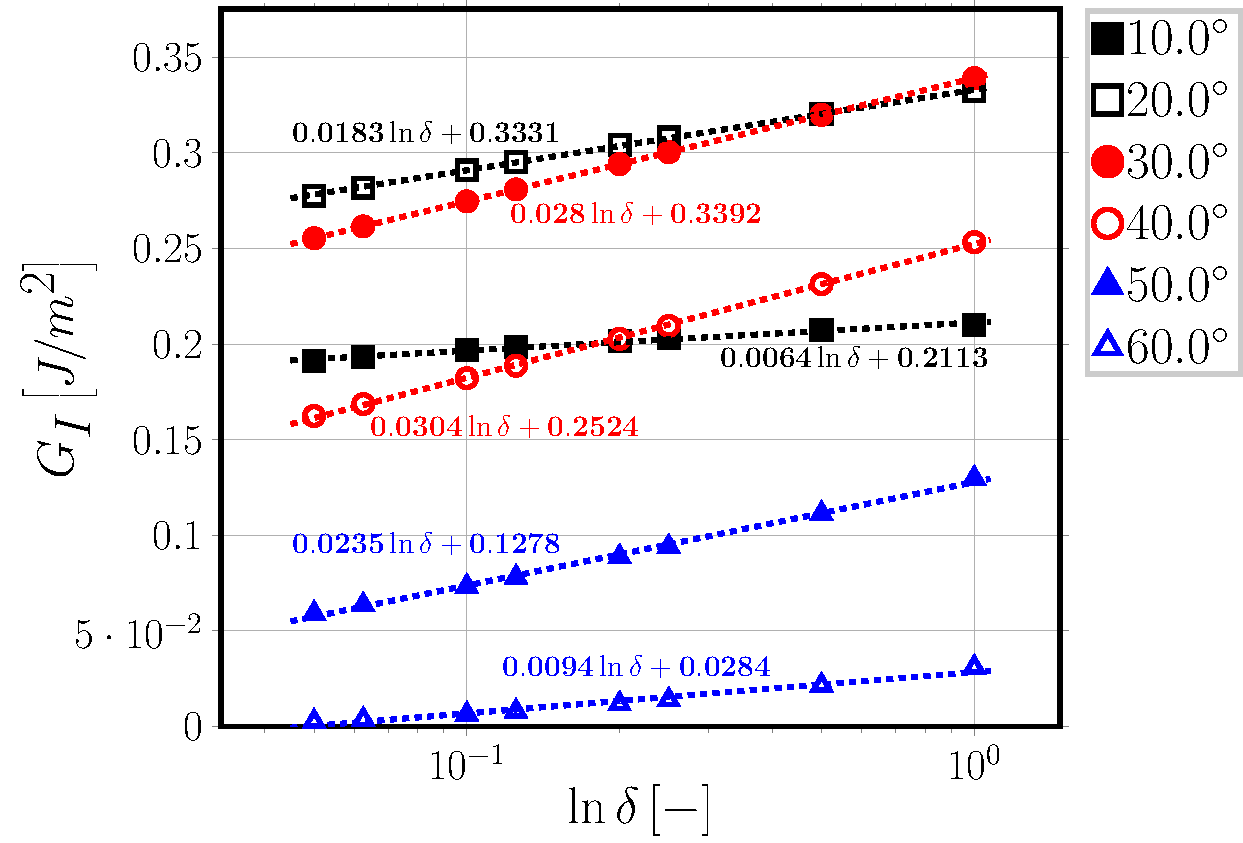
\includegraphics[width=\textwidth]{paperA/Vf0_1-free-1st-semilogvsDelta-GI.pdf}
       \caption{$V_{f}=0.1\%$, $1^{st}$ order elements.}
    \end{subfigure}
    ~
    \begin{subfigure}[b]{0.48\textwidth}
        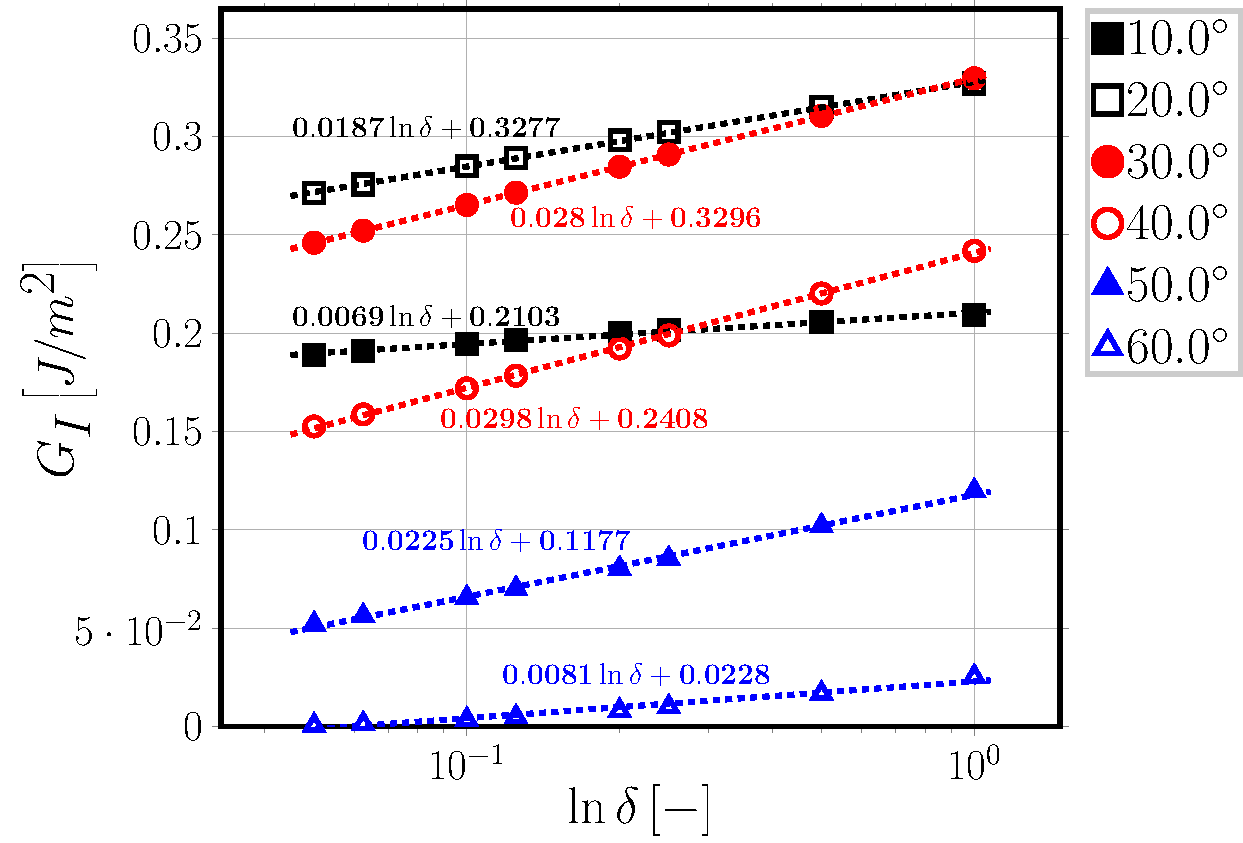
\includegraphics[width=\textwidth]{paperA/Vf0_1-free-2nd-semilogvsDelta-GI.pdf}
       \caption{$V_{f}=0.1\%$, $2^{nd}$ order elements.}
    \end{subfigure}

    \begin{subfigure}[b]{0.48\textwidth}
        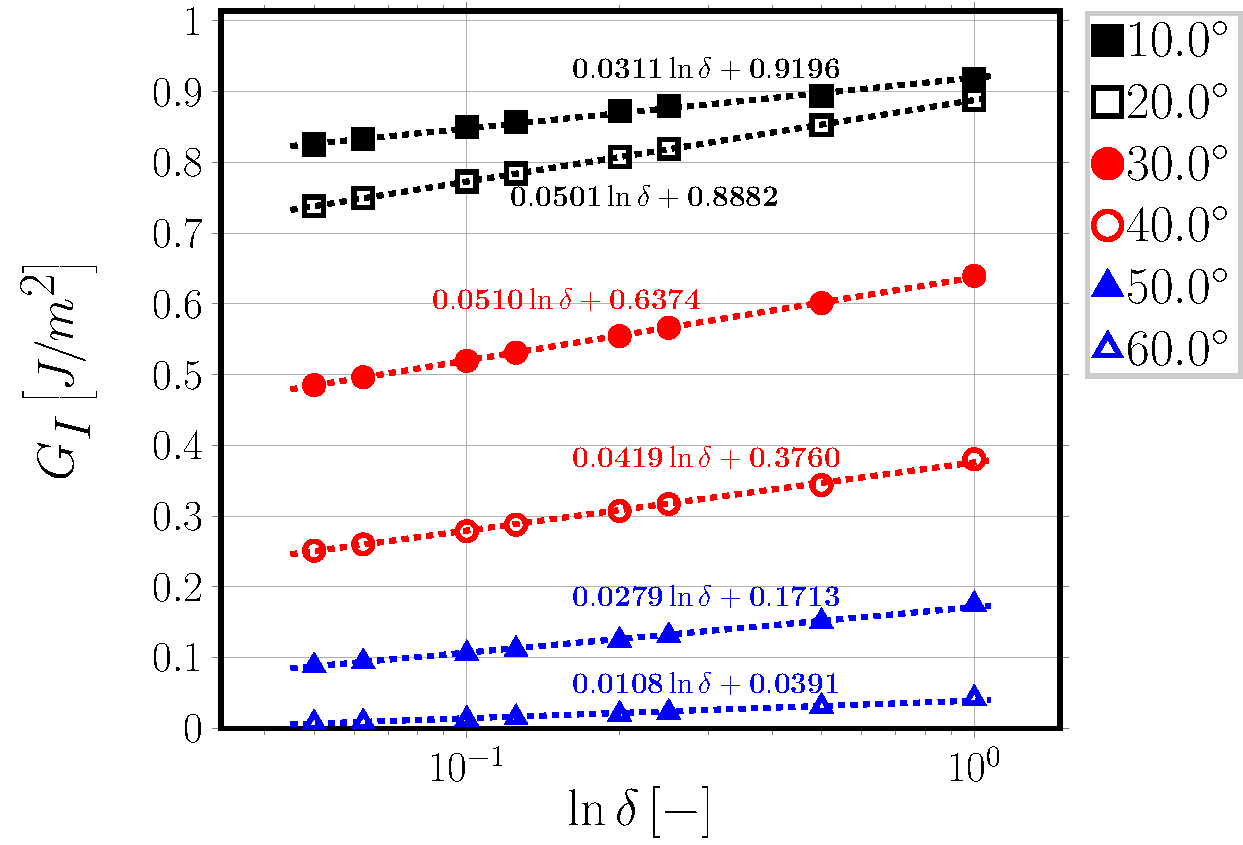
\includegraphics[width=\textwidth]{paperA/Vf40-free-1st-semilogvsDelta-GI.pdf}
       \caption{$V_{f}=40\%$, $1^{st}$ order elements.}
    \end{subfigure}
    ~
    \begin{subfigure}[b]{0.48\textwidth}
        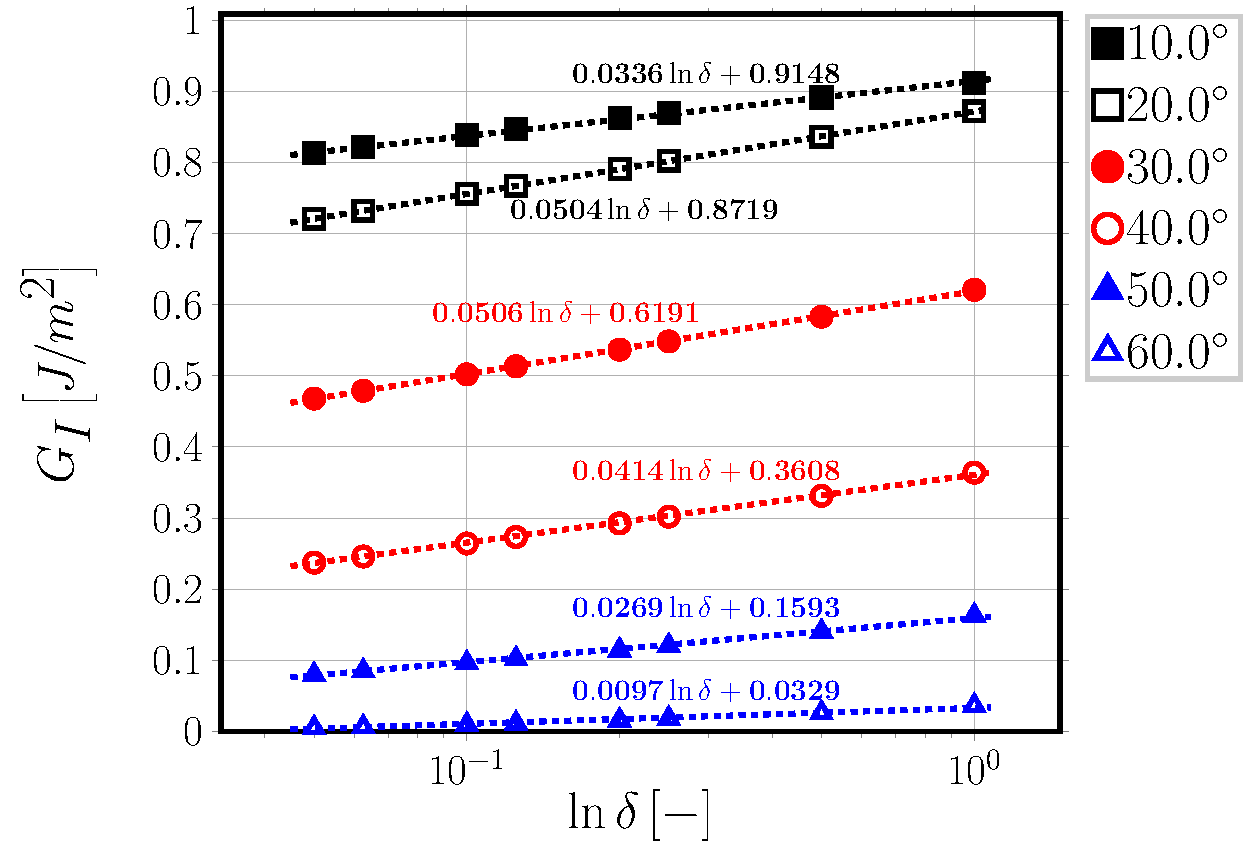
\includegraphics[width=\textwidth]{paperA/Vf40-free-2nd-semilogvsDelta-GI.pdf}
       \caption{$V_{f}=40\%$, $2^{nd}$ order elements.}
    \end{subfigure}

\caption{Logarithmic dependence on $\delta$ of Mode I ERR: interpolation of numerical results.}\label{chap3:paperA:fig:gIinterp}
\end{figure}

\begin{figure}[!h]
\centering
    \begin{subfigure}[b]{0.48\textwidth}
        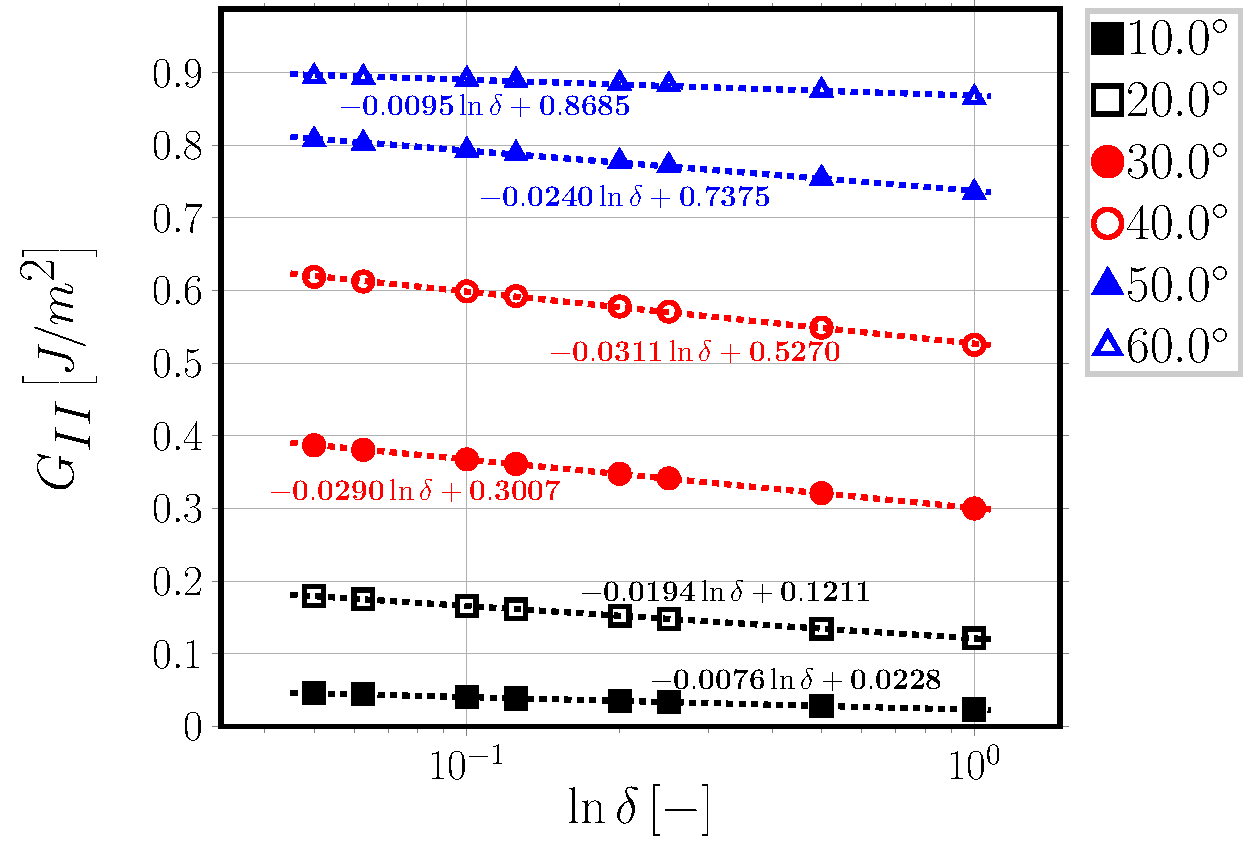
\includegraphics[width=\textwidth]{paperA/Vf0_1-free-1st-semilogvsDelta-GII.pdf}
       \caption{$V_{f}=0.1\%$, $1^{st}$ order elements.}
    \end{subfigure}
    ~
    \begin{subfigure}[b]{0.48\textwidth}
        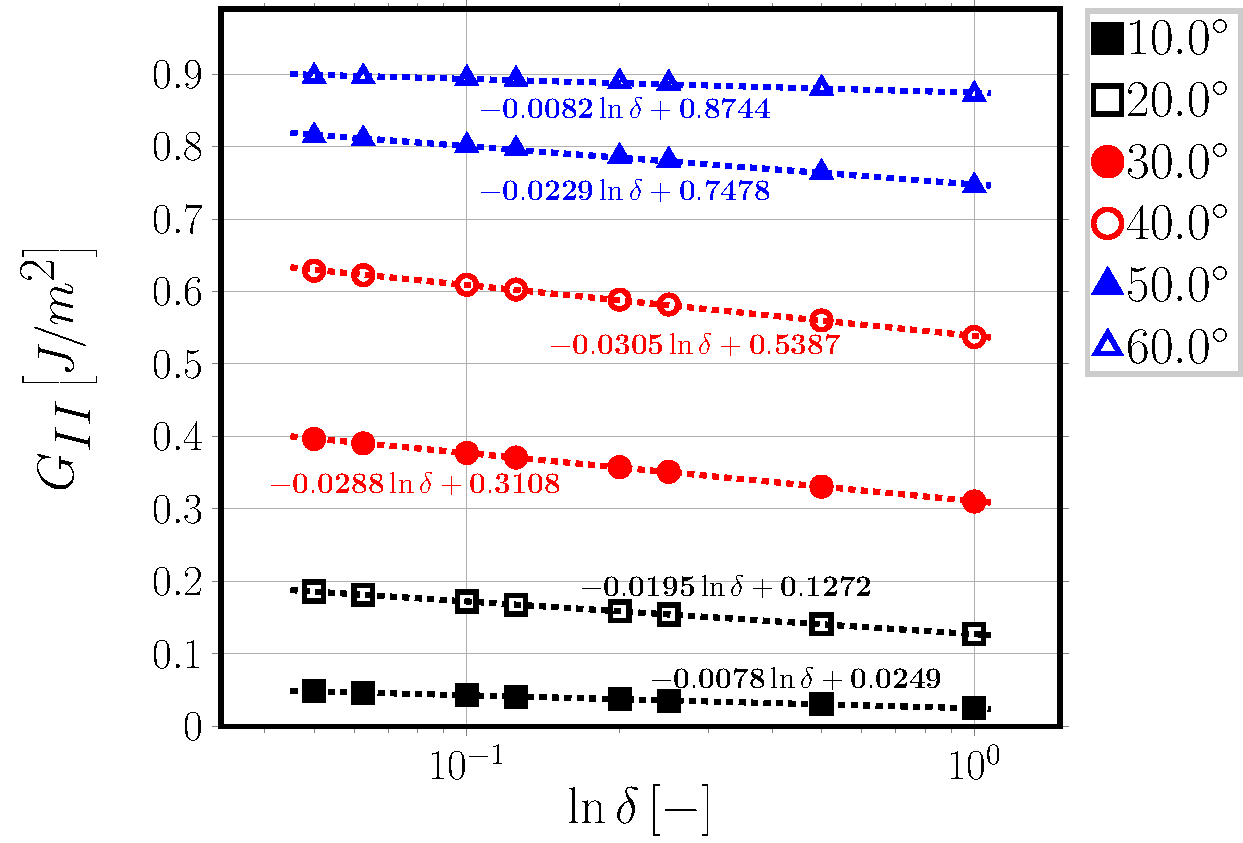
\includegraphics[width=\textwidth]{paperA/Vf0_1-free-2nd-semilogvsDelta-GII.pdf}
       \caption{$V_{f}=0.1\%$, $2^{nd}$ order elements.}
    \end{subfigure}

    \begin{subfigure}[b]{0.48\textwidth}
        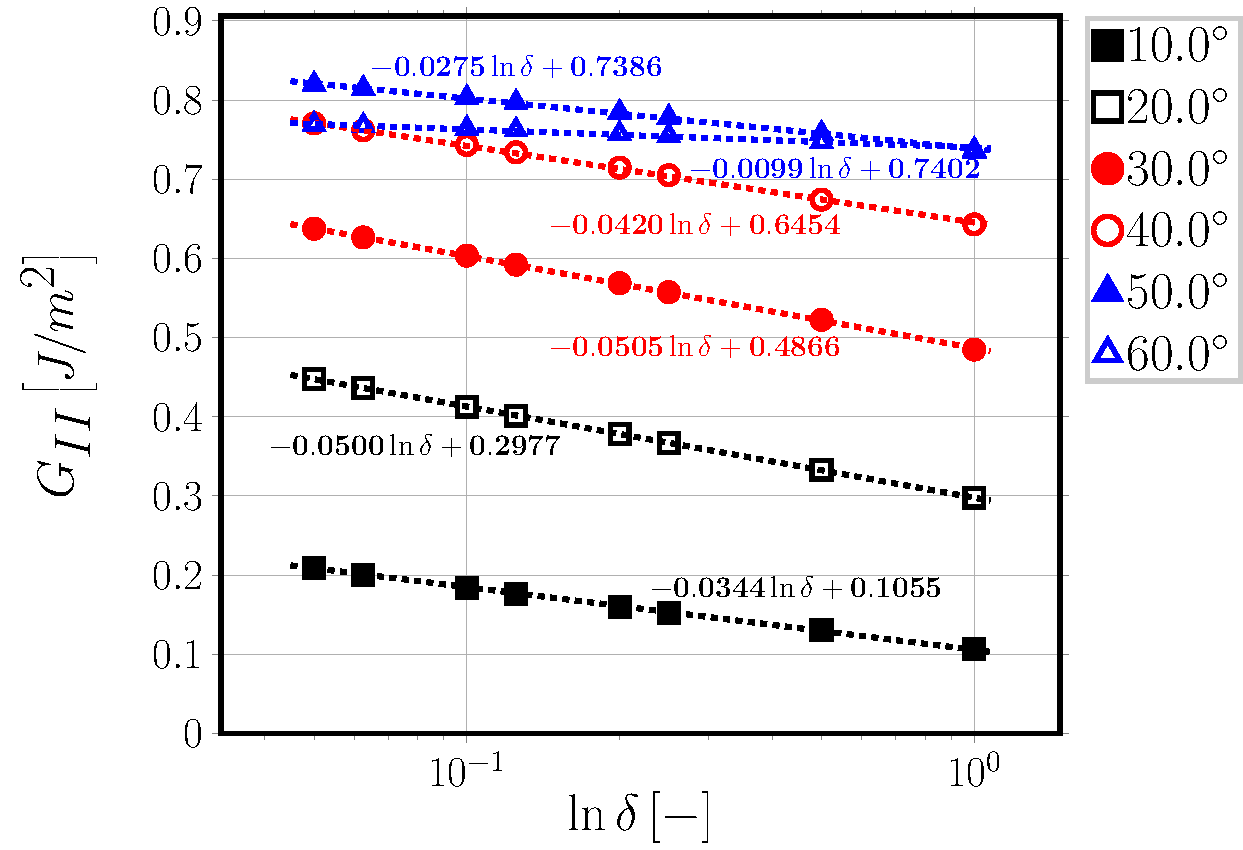
\includegraphics[width=\textwidth]{paperA/Vf40-free-1st-semilogvsDelta-GII.pdf}
       \caption{$V_{f}=40\%$, $1^{st}$ order elements.}
    \end{subfigure}
    ~
    \begin{subfigure}[b]{0.48\textwidth}
        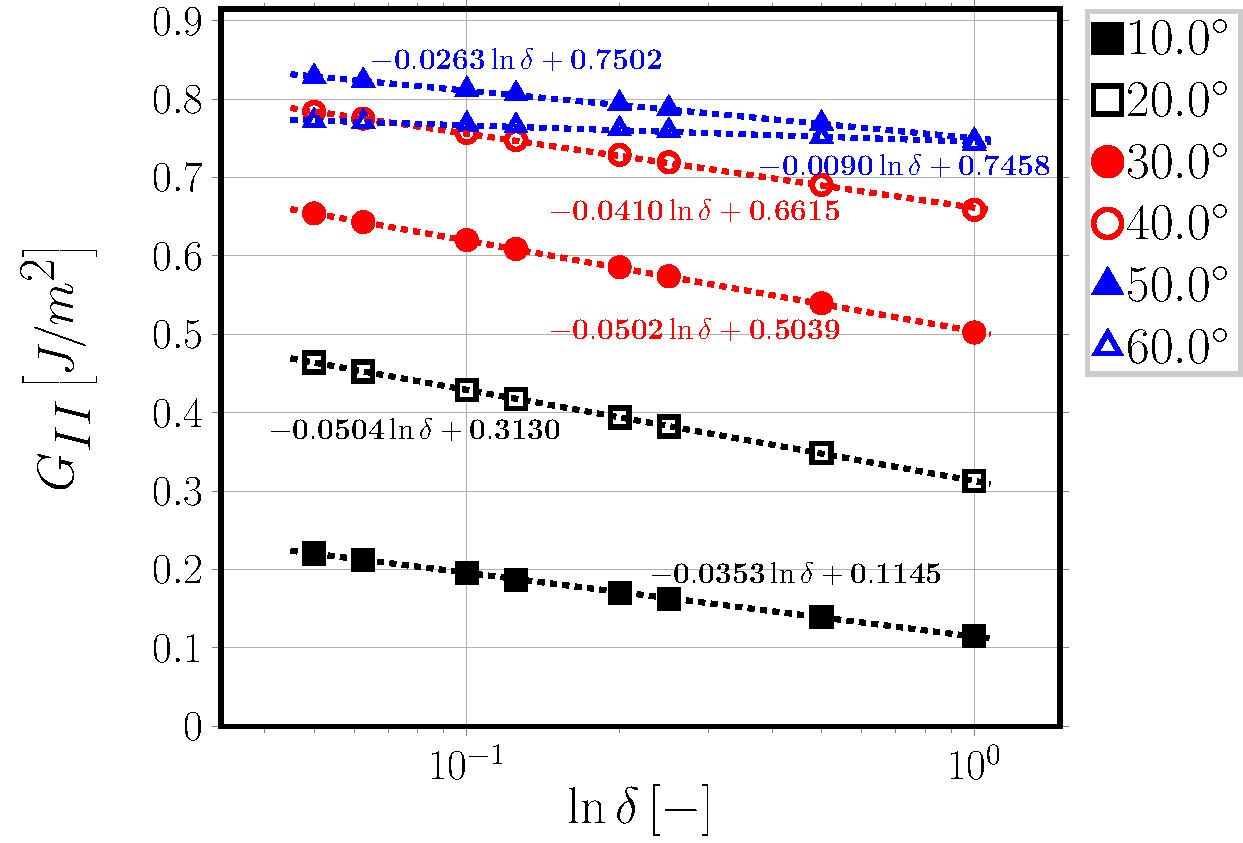
\includegraphics[width=\textwidth]{paperA/Vf40-free-2nd-semilogvsDelta-GII.pdf}
       \caption{$V_{f}=40\%$, $2^{nd}$ order elements.}
    \end{subfigure}

\caption{Logarithmic dependence on $\delta$ of Mode II ERR: interpolation of numerical results.}\label{chap3:paperA:fig:gIIinterp}
\end{figure}

It is found in Paper A that

\begin{itemize}
\item the total Ener is invariant to rotations of the reference frame (and more in general to linear transformations), which implies that rotation of crack tip forces and displacement is actually not required in the use of the VCCT for the calculation of $G_{TOT}$;
\item the total ERR does not depend on the size $\delta$ of the elements at the crack tip, at least for reasonably small elements ($\delta\leq1.0^{\circ}$) ;
\item as a consequence, Mode II ERR for the \emph{closed} interface crack does not depend on $\delta$, as $G_{II}=G_{TOT}$ after the onset of the contact zone;
\item for the \emph{open} interface crack, Mode I and Mode II ERR depend on the element size $\delta$ through a logarithmic law of the type $A\left(\Delta\theta\right)\ln\delta+B\left(\Delta\theta\right)$, as shown in Figure~\ref{chap3:paperA:fig:gIinterp} and Figure~\ref{chap3:paperA:fig:gIIinterp};
\item the sign of the logarithm is always positive for $G_{I}$ (see Figure~\ref{chap3:paperA:fig:gIinterp}), i.e. it decreases when $\delta$ decreases, and negative for $G_{II}$ (see Figure~\ref{chap3:paperA:fig:gIIinterp}), i.e. it increases when $\delta$ decreases.
\end{itemize}


%%%%%%%%%%%%%%%%%%%%%%%%%%%%%%%%%%%%%%%%%%%%%%%%%%%%%%%%%%%%%%%%%%%%%%%
%      Paper B
%%%%%%%%%%%%%%%%%%%%%%%%%%%%%%%%%%%%%%%%%%%%%%%%%%%%%%%%%%%%%%%%%%%%%%%
\section{Paper B}
\section*{Energy release rate of the fiber/matrix interface crack in UD composites under transverse loading: effect of the fiber volume fraction and of the distance to the free surface and to non-adjacent debonds}

In Paper B, fiber/matrix interface crack growth is studied in Representative Volume Elements of UD composites subjected to transverse tensile loading. A unit cell constituted by one fiber and the surrounding matrix, shown in Figure~\ref{chap3:paperB:fig:modelschem}, represents the basic element of the RVE.

\begin{figure}[!h]
    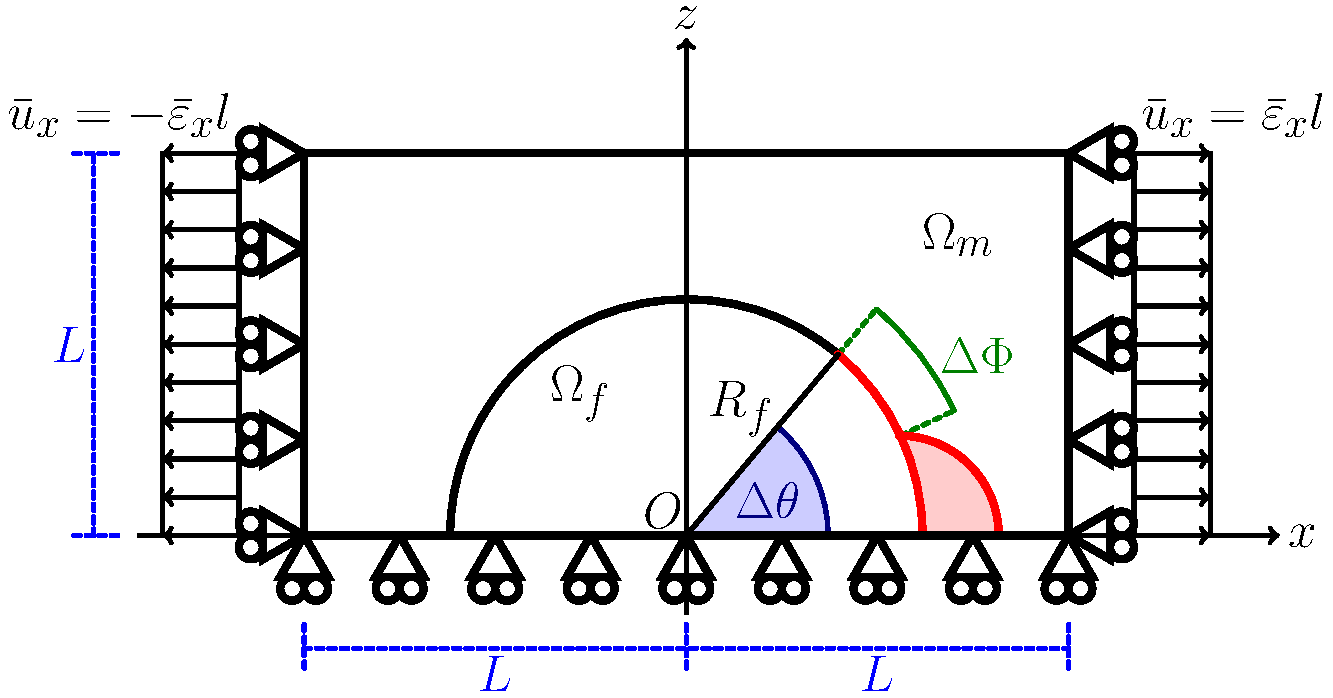
\includegraphics[width=0.9\textwidth]{paperB/RUC.pdf}
    \caption{Schematic of the reference unit cell with its main parameters.}\label{chap3:paperB:fig:modelschem}
\end{figure}

The unit cell has a size of $2L\times2L$, where

\begin{equation}\label{chap3:paperB:eq:LVf}
L=\frac{R_{f}}{2}\sqrt{\frac{\pi}{V_{f}}},
\end{equation}

$R_{f}$ is the fiber radius, assumed to be equal to $1\ \mu m$, and $V_{f}$ is the fiber volume fraction. Notice that the value of $1\ \mu m$ for the fiber radius is arbitrary and chosen for simplicity: in the context of Linear Elastic Fracture Mechanics (LEFM), the Energy Release Rate (ERR) is directly proportional to the fiber radius, thus evaluation of the ERR for another value requires simply a multiplication.\\
The RVE is made up by $n$ unit cells as the one of Figure~\ref{chap3:paperB:fig:modelschem} in the horizontal (loading) direction and $k$ unit cells in the vertical (through-the-thickness) direction (see Figure~\ref{chap3:paperB:fig:thickply}). The fiber of the unit cell placed in the center of the RVE is always partially debonded, and the debond has an angular size $\Delta\theta$ which can vary between $10^{\circ}$ and $150^{\circ}$.

\begin{figure}[!h]
    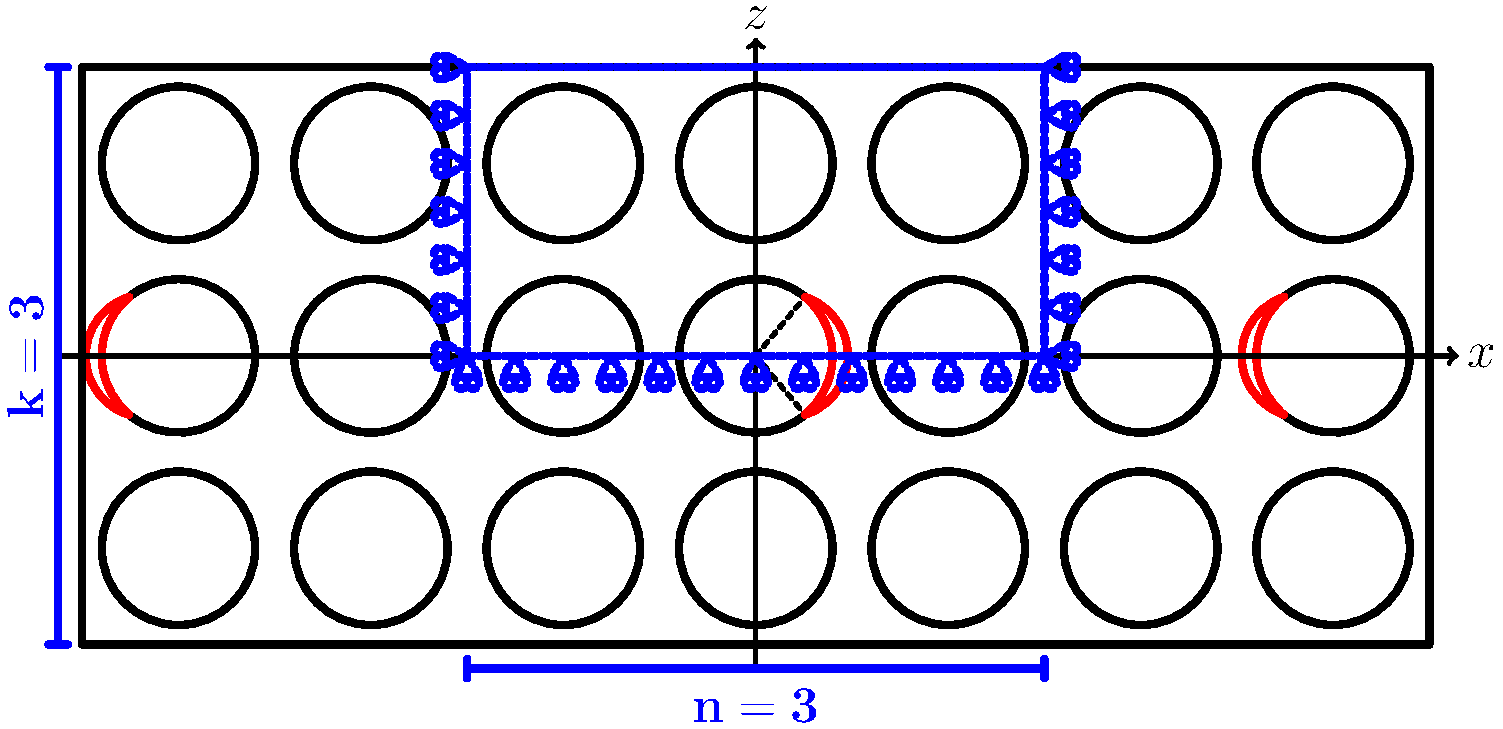
\includegraphics[width=0.9\textwidth]{paperB/thickPly.pdf}
    \caption{Multiple rows of fibers with a debond appearing every $n$ fibers within the central row: model $n\times k-free$ ($n=3$ and $k=3$ in the figure).}\label{chap3:paperB:fig:thickply}
\end{figure}

The RVE is symmetric with respect to the horizontal axis ($x$-axis), thus only half of it is explicitly modelled and conditions of symmetry are applied on the lower boundary of the RVE. On the left and right boundaries, conditions of coupling of the $x$-displacement (horizontal displacement) are applied. This implies that the computed solution corresponds to the RVE repeating an infinite number of times to the left and to the right symmetrically with the respect to the side boundary, i.e. if the debond in the central unit cell is placed on the right side of the fiber, then the next one to the right and to the left is on the left side, the successive one is on the right, and so on. As a consequence, the number $n$ of unit cells in the horizontal direction determines the distance between consecutive debonds in the horizontal direction, which corresponds to $n-1$ fully bonded fibers. The upper and lower boundaries (but, given the symmetry with respect to the $x$-axis, only the upper one is explicitly modeled) are left free. Thus, the family of RVEs studied in this paper is called $n\times k-free$.\\
A constant $x$-strain equal to $1\%$ is applied to the left and right boundary. The selected value of $1\%$ is arbitrary, as in LEFM the ERR is proportional to the square of the strain. Thus, the value of the ERR for another level of applied strain can calculated with a multiplication. Contact between debond faces is considered frictionless. The fiber and matrix phases, respectively glass fiber and epoxy, are considered to be homogeneous, isotropic and linear elastic. Their material properties are reported in Table~\ref{chap3:paperB:tab:phaseprop}.

\begin{table}[!htbp]
 \centering
 \caption{Summary of the mechanical properties of fiber and matrix. $E$ stands for Young's modulus, $\mu$ for shear modulus and $\nu$ for Poisson's ratio.}
 \begin{tabular}{cccc}
\\
\textbf{Material} & \textbf{$E\left[GPa\right]$}\ & \textbf{$\mu\left[GPa\right]$} & \textbf{$\nu\left[-\right]$} \\
\midrule
Glass fiber    & 70.0  & 29.2   & 0.2  \\
Epoxy    & 3.5    & 1.25   & 0.4
\end{tabular}
\label{chap3:paperB:tab:phaseprop}
\end{table}

The model is meshed with second order quadrilateral and triangular elements, while at the crack tip only second order quadrilateral elements are used with unitary aspect ratio, determined by the arc size $R_{f}\delta$ where $\delta$ is the angular size. Given the results on convergence of Paper A, the angular size $\delta$ of the elements at the crack tip is determined here by comparison with the Boundary Element Method (BEM) results provided in~\cite{Paris2007,Sandino2016} for a single debonded fiber in an infinite matrix. The comparison is conducted using the $1\times1-free$ RVE with $V_{f}=0.0079$, which corresponds to $L\sim100 R_{f}$. A trade-off between accuracy and computational cost (time and memory required for the solution) is found for $\delta=0.05^{\circ}$. A comparison between the ERR computed with $\delta=0.05^{\circ}$ and the BEM results is shown in Figure~\ref{chap3:paperB:fig:validation}. The error between FEM and BEM solution does not exceed $5\%$ for any value of $\Delta\theta$. This provides a measure of the accuracy of the results proposed here: differences between values of ERR smaller than $5\%$ should not be taken into consideration.

\begin{figure}[!h]
\centering
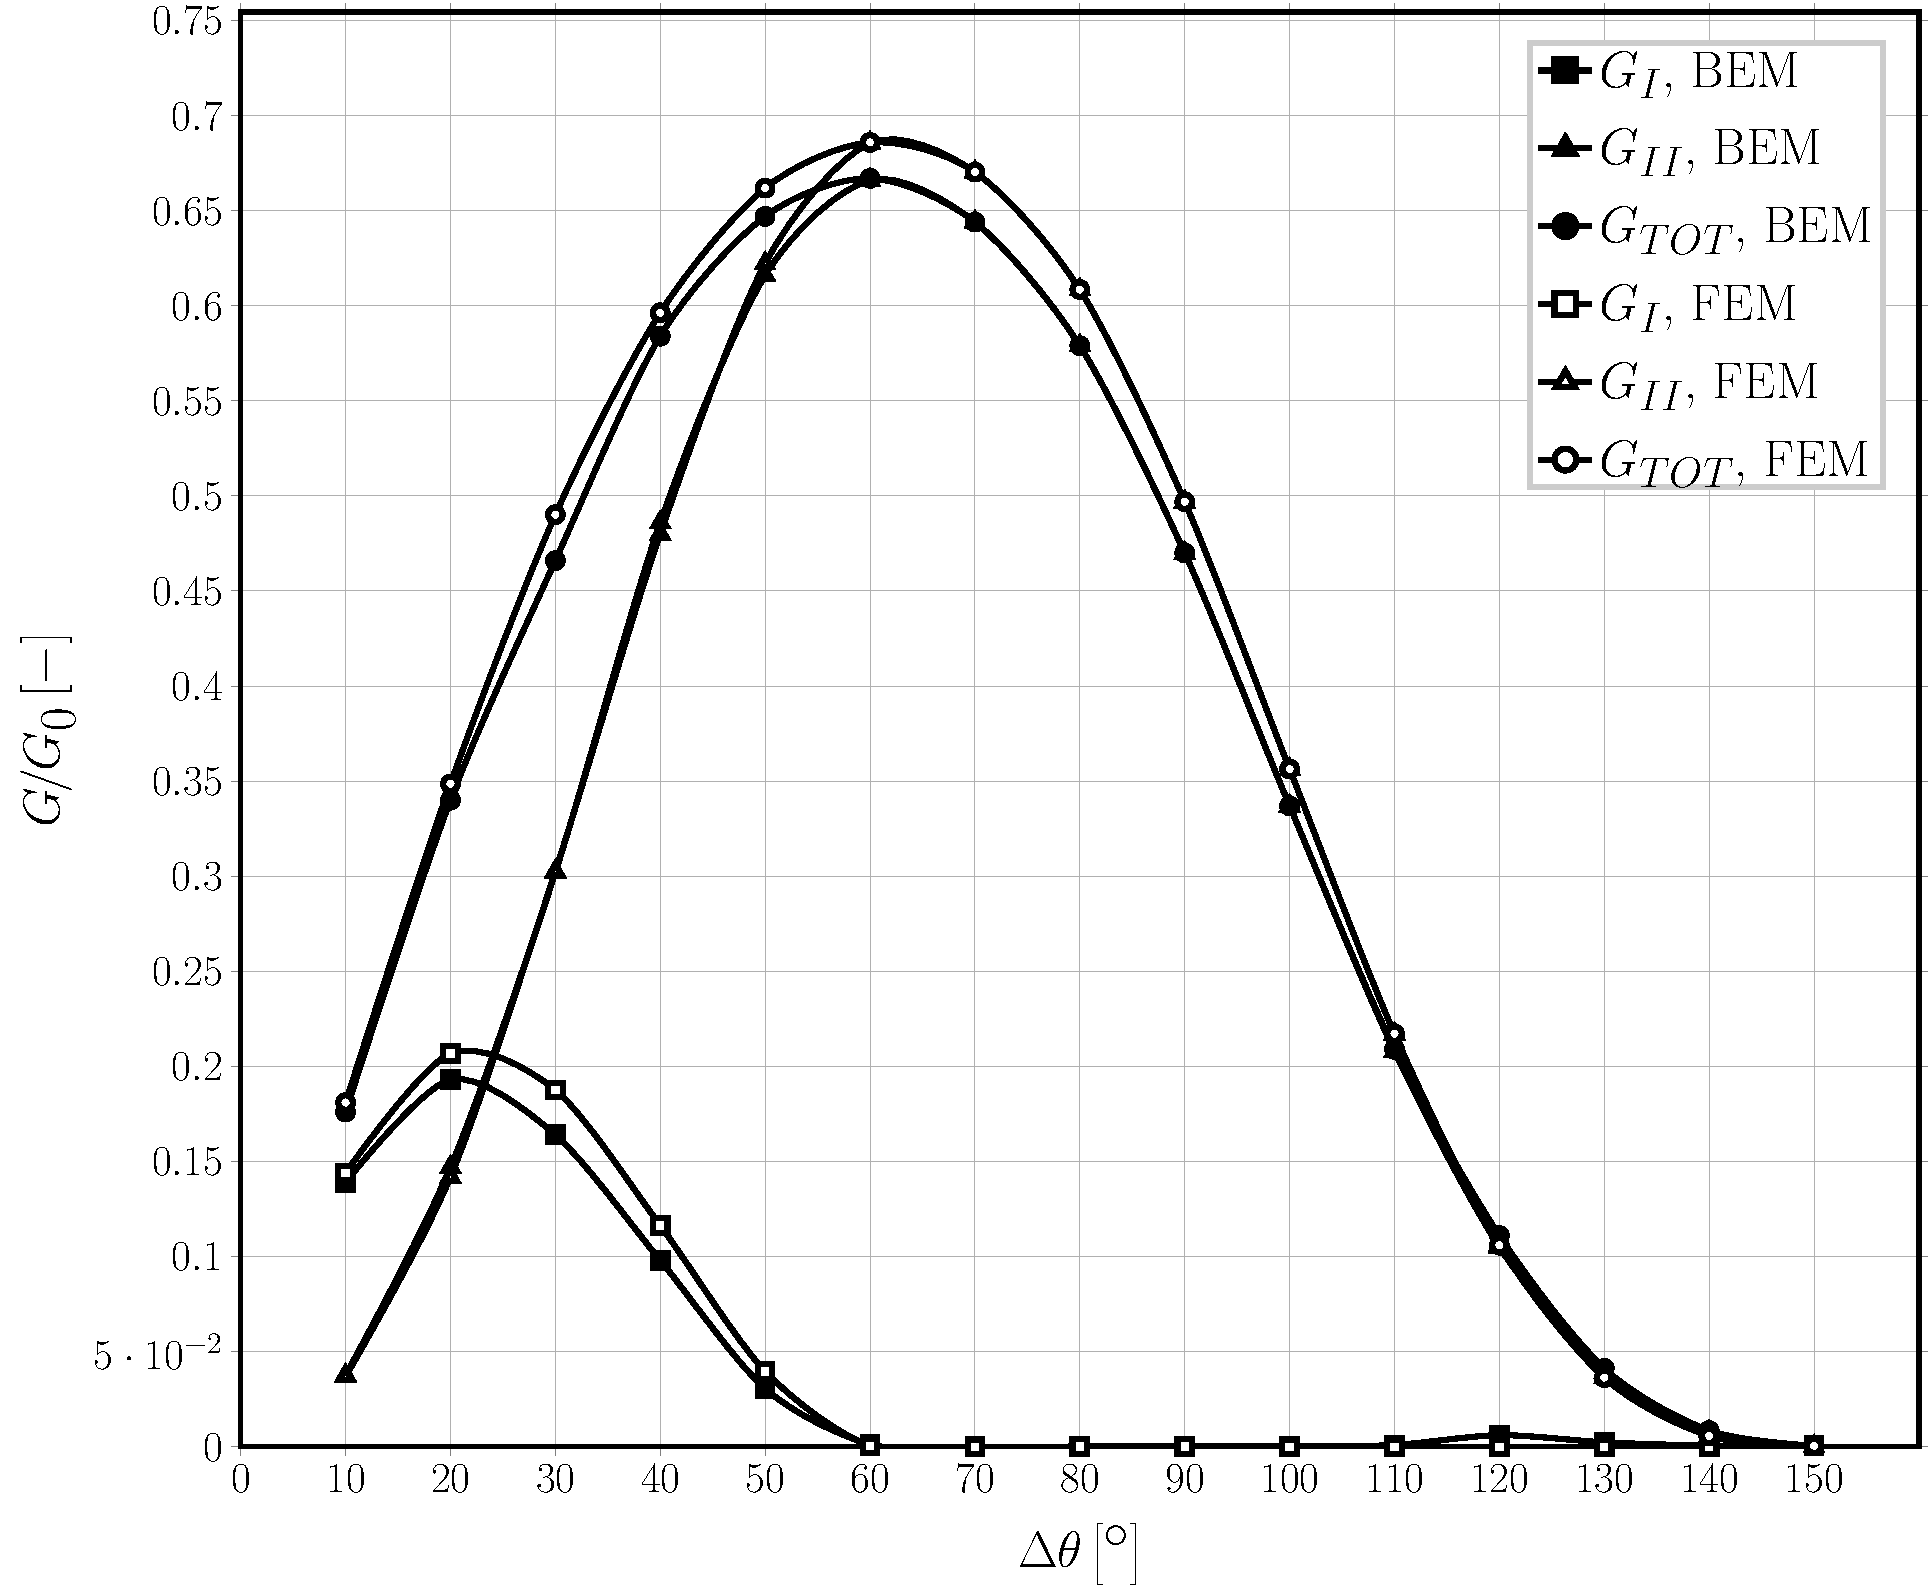
\includegraphics[width=0.9\textwidth]{paperB/validation-VCCT.pdf}
\caption{Validation of the single fiber model for the infinite matrix case with respect to the BEM solution in \cite{Sandino2016}.}\label{chap3:paperB:fig:validation}
\end{figure}

The most important observations and conclusions of the paper are summarized below.

\begin{enumerate}
\item The Energy Release Rate, both Mode I and Mode II, decreases with a decreasing number of fully bonded fibers between two consecutive partially debonded fibers in the central row, as shown in Figure~\ref{chap3:paperB:fig:sidefibersMI} for Mode I and Figure~\ref{chap3:paperB:fig:sidefibersMI} for Mode II in the case of $n\times1-free$ RVE. Furthermore, it seems that a characteristic distance between debonds exits that defines the transition between an interactive and a non-interactive solution. However, this distance appears to depend on the thickness of the UD, i.e. on the number $k$ of fiber rows in the vertical direction, and also on the fiber volume fraction. An estimate of such distance provides: around $100$ fully bonded fibers for a 1-fiber-row thick UD with $V_{f}=30\%$; around $200$ fibers for a 1-fiber-row thick UD with $V_{f}=60\%$; around $100$ fibers for a 5-fibers-row thick UD with $V_{f}=60\%$.
\item When the free surface is close to the debond, higher Mode I and Mode II ERRs are obtained and the peak $G$ values are shifted to larger debonds (Figure~\ref{chap3:paperB:fig:sidefibersMI} and Figure~\ref{chap3:paperB:fig:sidefibersMI}). However, the effect of the composite free surface on the ERR declines very fast: the presence of at least $2$ fully bonded fibers below and above the central row results in stable constant values of ERR.
\item An increase in the fiber volume fraction, which corresponds to a decrease in the inter-fiber distance, leads in general to a magnification of the effects previously described.
\end{enumerate}

\begin{figure}[!h]
\centering
    \begin{subfigure}[b]{0.475\textwidth}
        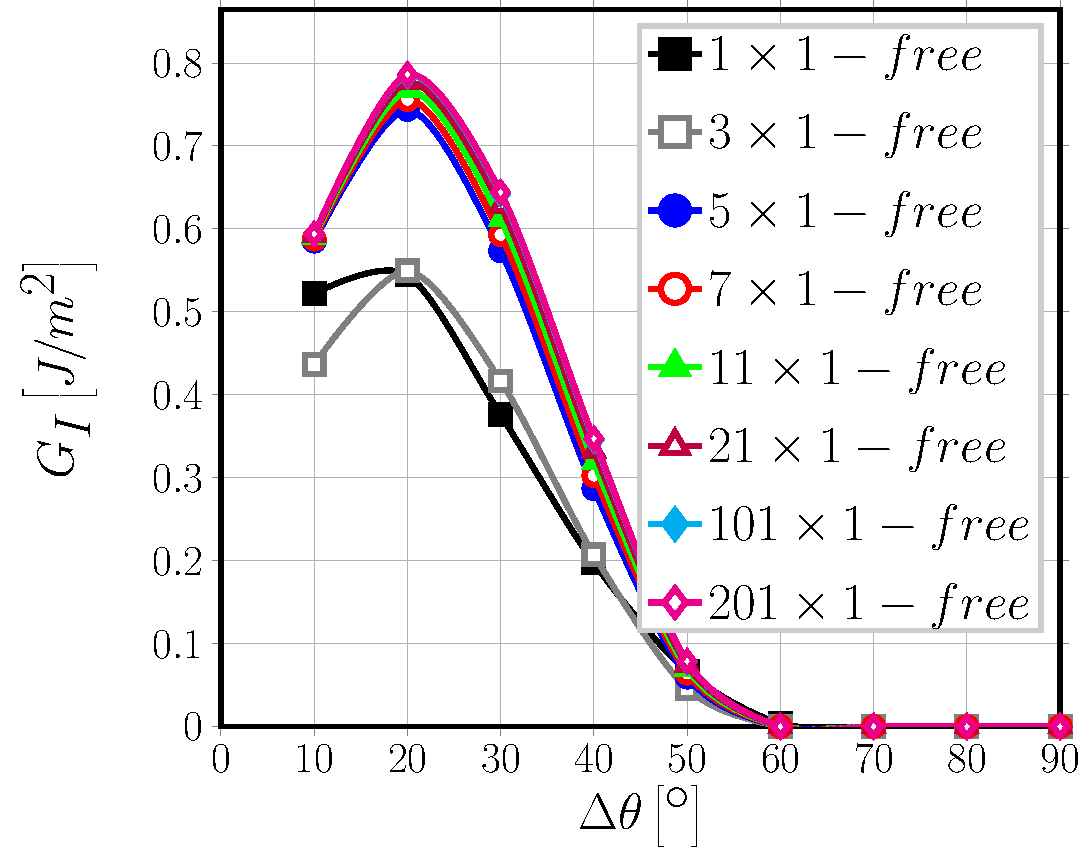
\includegraphics[width=\textwidth]{paperB/sidefibers-vf30-GI.pdf}
        \caption{$V_{f}=30\%$.}\label{chap3:paperB:subfig:sidefiber30MI}
    \end{subfigure} ~
    \begin{subfigure}[b]{0.475\textwidth}
        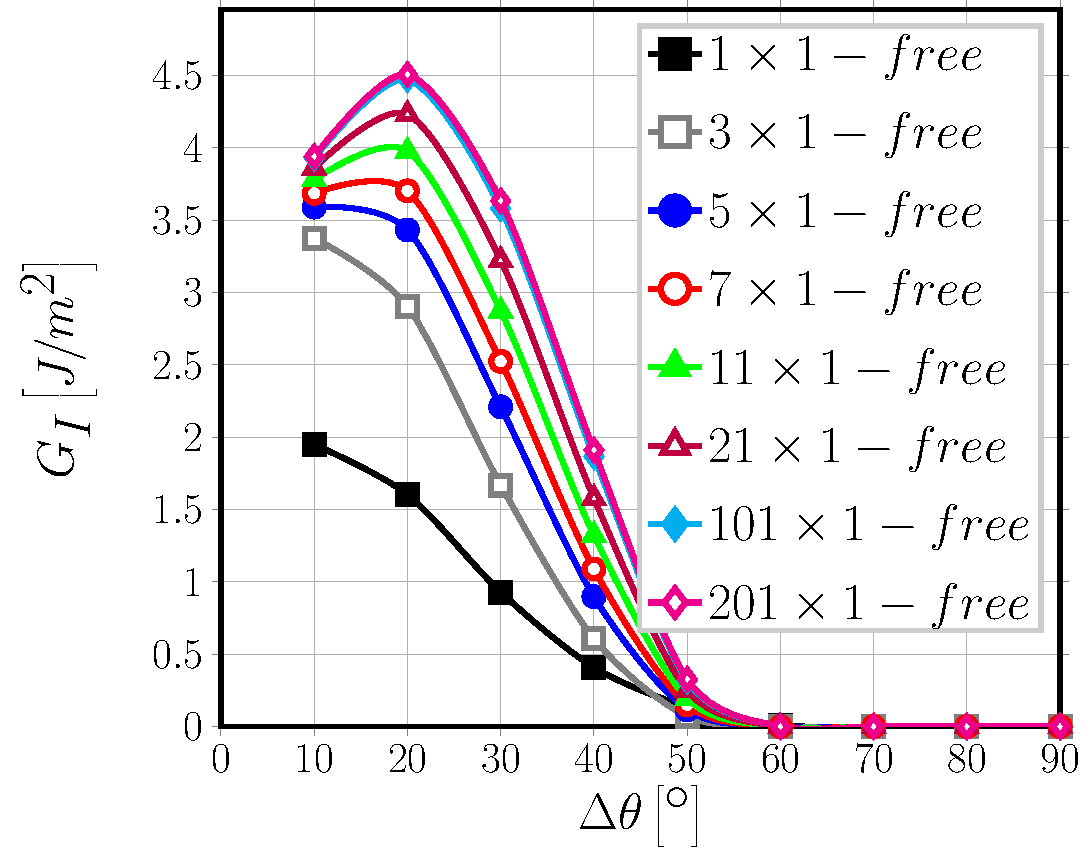
\includegraphics[width=\textwidth]{paperB/sidefibers-vf60-GI.pdf}
        \caption{$V_{f}=60\%$.}\label{chap3:paperB:subfig:sidefiber60MI}
    \end{subfigure}

\caption{Effect of the interaction between debonds appearing at regular intervals on Mode I ERR in an UD with a single row of fibers at different levels of fiber volume fraction $V_{f}$, subject to an applied transverse strain $\varepsilon_{x}$ of $1\%$.}\label{chap3:paperB:fig:sidefibersMI}
\end{figure}

\begin{figure}[!h]
\centering
    \begin{subfigure}[b]{0.475\textwidth}
        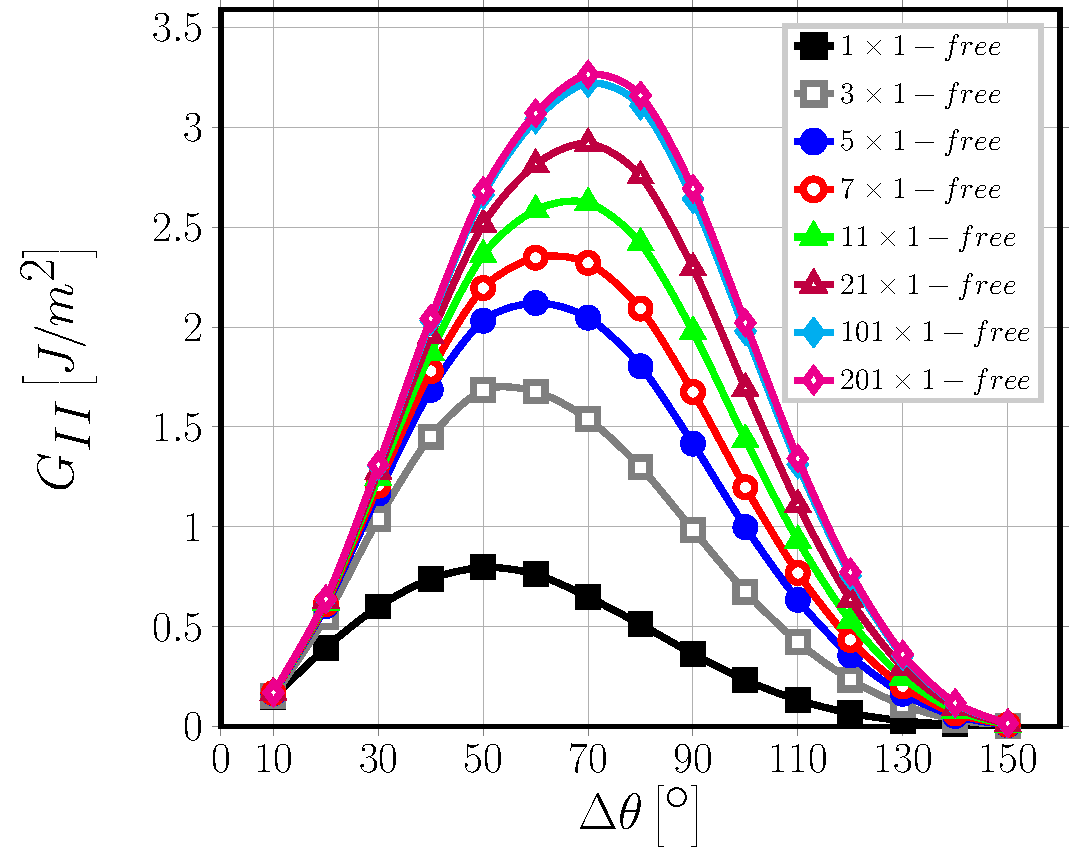
\includegraphics[width=\textwidth]{paperB/sidefibers-vf30-GII.pdf}
        \caption{$V_{f}=30\%$.}\label{chap3:paperB:subfig:sidefiber30MII}
    \end{subfigure} ~
    \begin{subfigure}[b]{0.475\textwidth}
        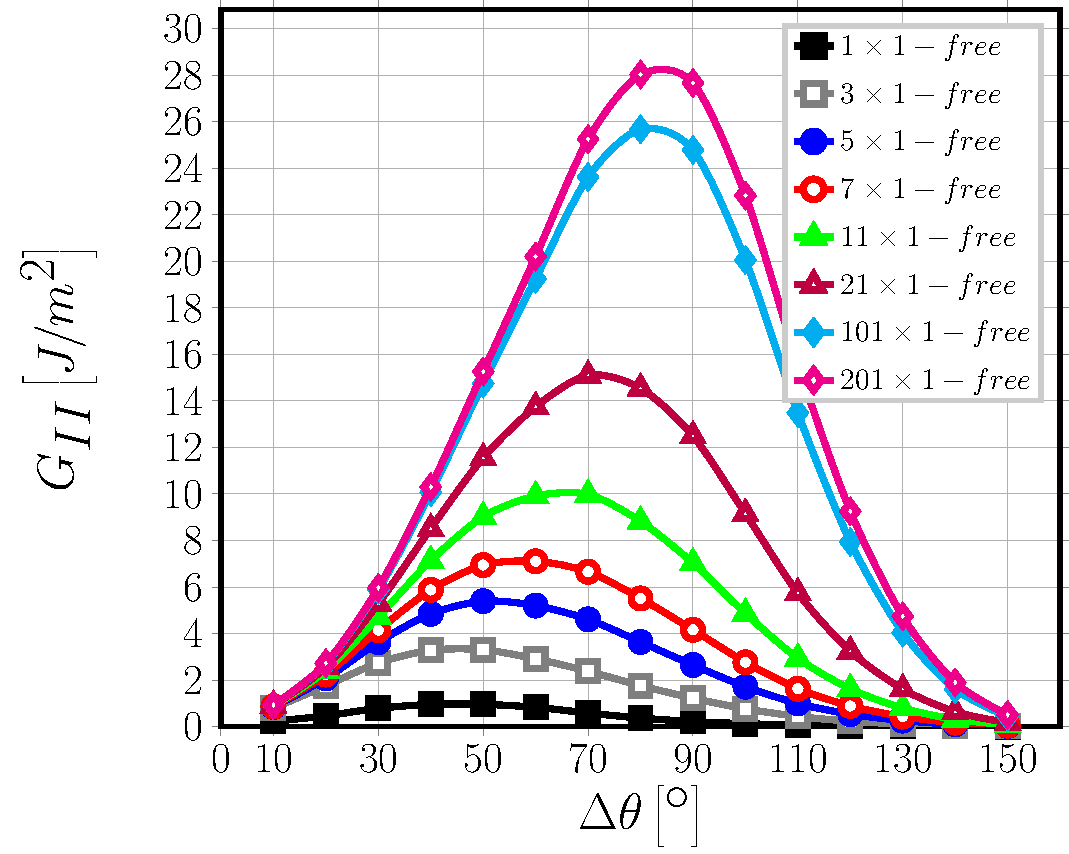
\includegraphics[width=\textwidth]{paperB/sidefibers-vf60-GII.pdf}
        \caption{$V_{f}=60\%$.}\label{chap3:paperB:subfig:sidefiber60MII}
    \end{subfigure}

\caption{Effect of the interaction between debonds appearing at regular intervals on Mode II ERR in an UD with a single row of fibers at different levels of fiber volume fraction $V_{f}$, subject to an applied transverse strain $\varepsilon_{x}$ of $1\%$.}\label{chap3:paperB:fig:sidefibersMII}
\end{figure}

%%%%%%%%%%%%%%%%%%%%%%%%%%%%%%%%%%%%%%%%%%%%%%%%%%%%%%%%%%%%%%%%%%%%%%%
%      Paper C
%%%%%%%%%%%%%%%%%%%%%%%%%%%%%%%%%%%%%%%%%%%%%%%%%%%%%%%%%%%%%%%%%%%%%%%
\section{Paper C}
\section*{Effect of the proximity to the $\mathbf{0^{\circ}/90^{\circ}}$ interface on Energy Release Rate of fiber/matrix interface crack growth in the  $\mathbf{90^{\circ}}$-ply of a cross-ply laminate under tensile loading}

In Paper C, fiber/matrix interface crack growth is studied in Representative Volume Elements of cross-ply laminates subjected to tensile loading. Similarly to Paper B, the unit cell constituted by one fiber and the surrounding matrix, shown in Figure~\ref{chap3:paperB:fig:modelschem}, represents the basic element of the RVE. The unit cell has a size of $2L\times2L$, where

\begin{equation}\label{chap3:paperC:eq:LVf}
L=\frac{R_{f}}{2}\sqrt{\frac{\pi}{V_{f}}},
\end{equation}

$R_{f}$ is the fiber radius, assumed again to be equal to $1\ \mu m$, and $V_{f}$ is the fiber volume fraction.\\
The RVE is constituted by $n$ unit cells in the horizontal (loading) direction and $k$ unit cells in the vertical (through-the-thickness) direction (see Figure~\ref{chap3:paperC:fig:laminateModelsB}). The fiber of the unit cell placed in the center of the RVE is always partially debonded, and the debond has an angular size $\Delta\theta$ which can vary between $10^{\circ}$ and $150^{\circ}$.

\begin{figure}[!htb]
\centering
        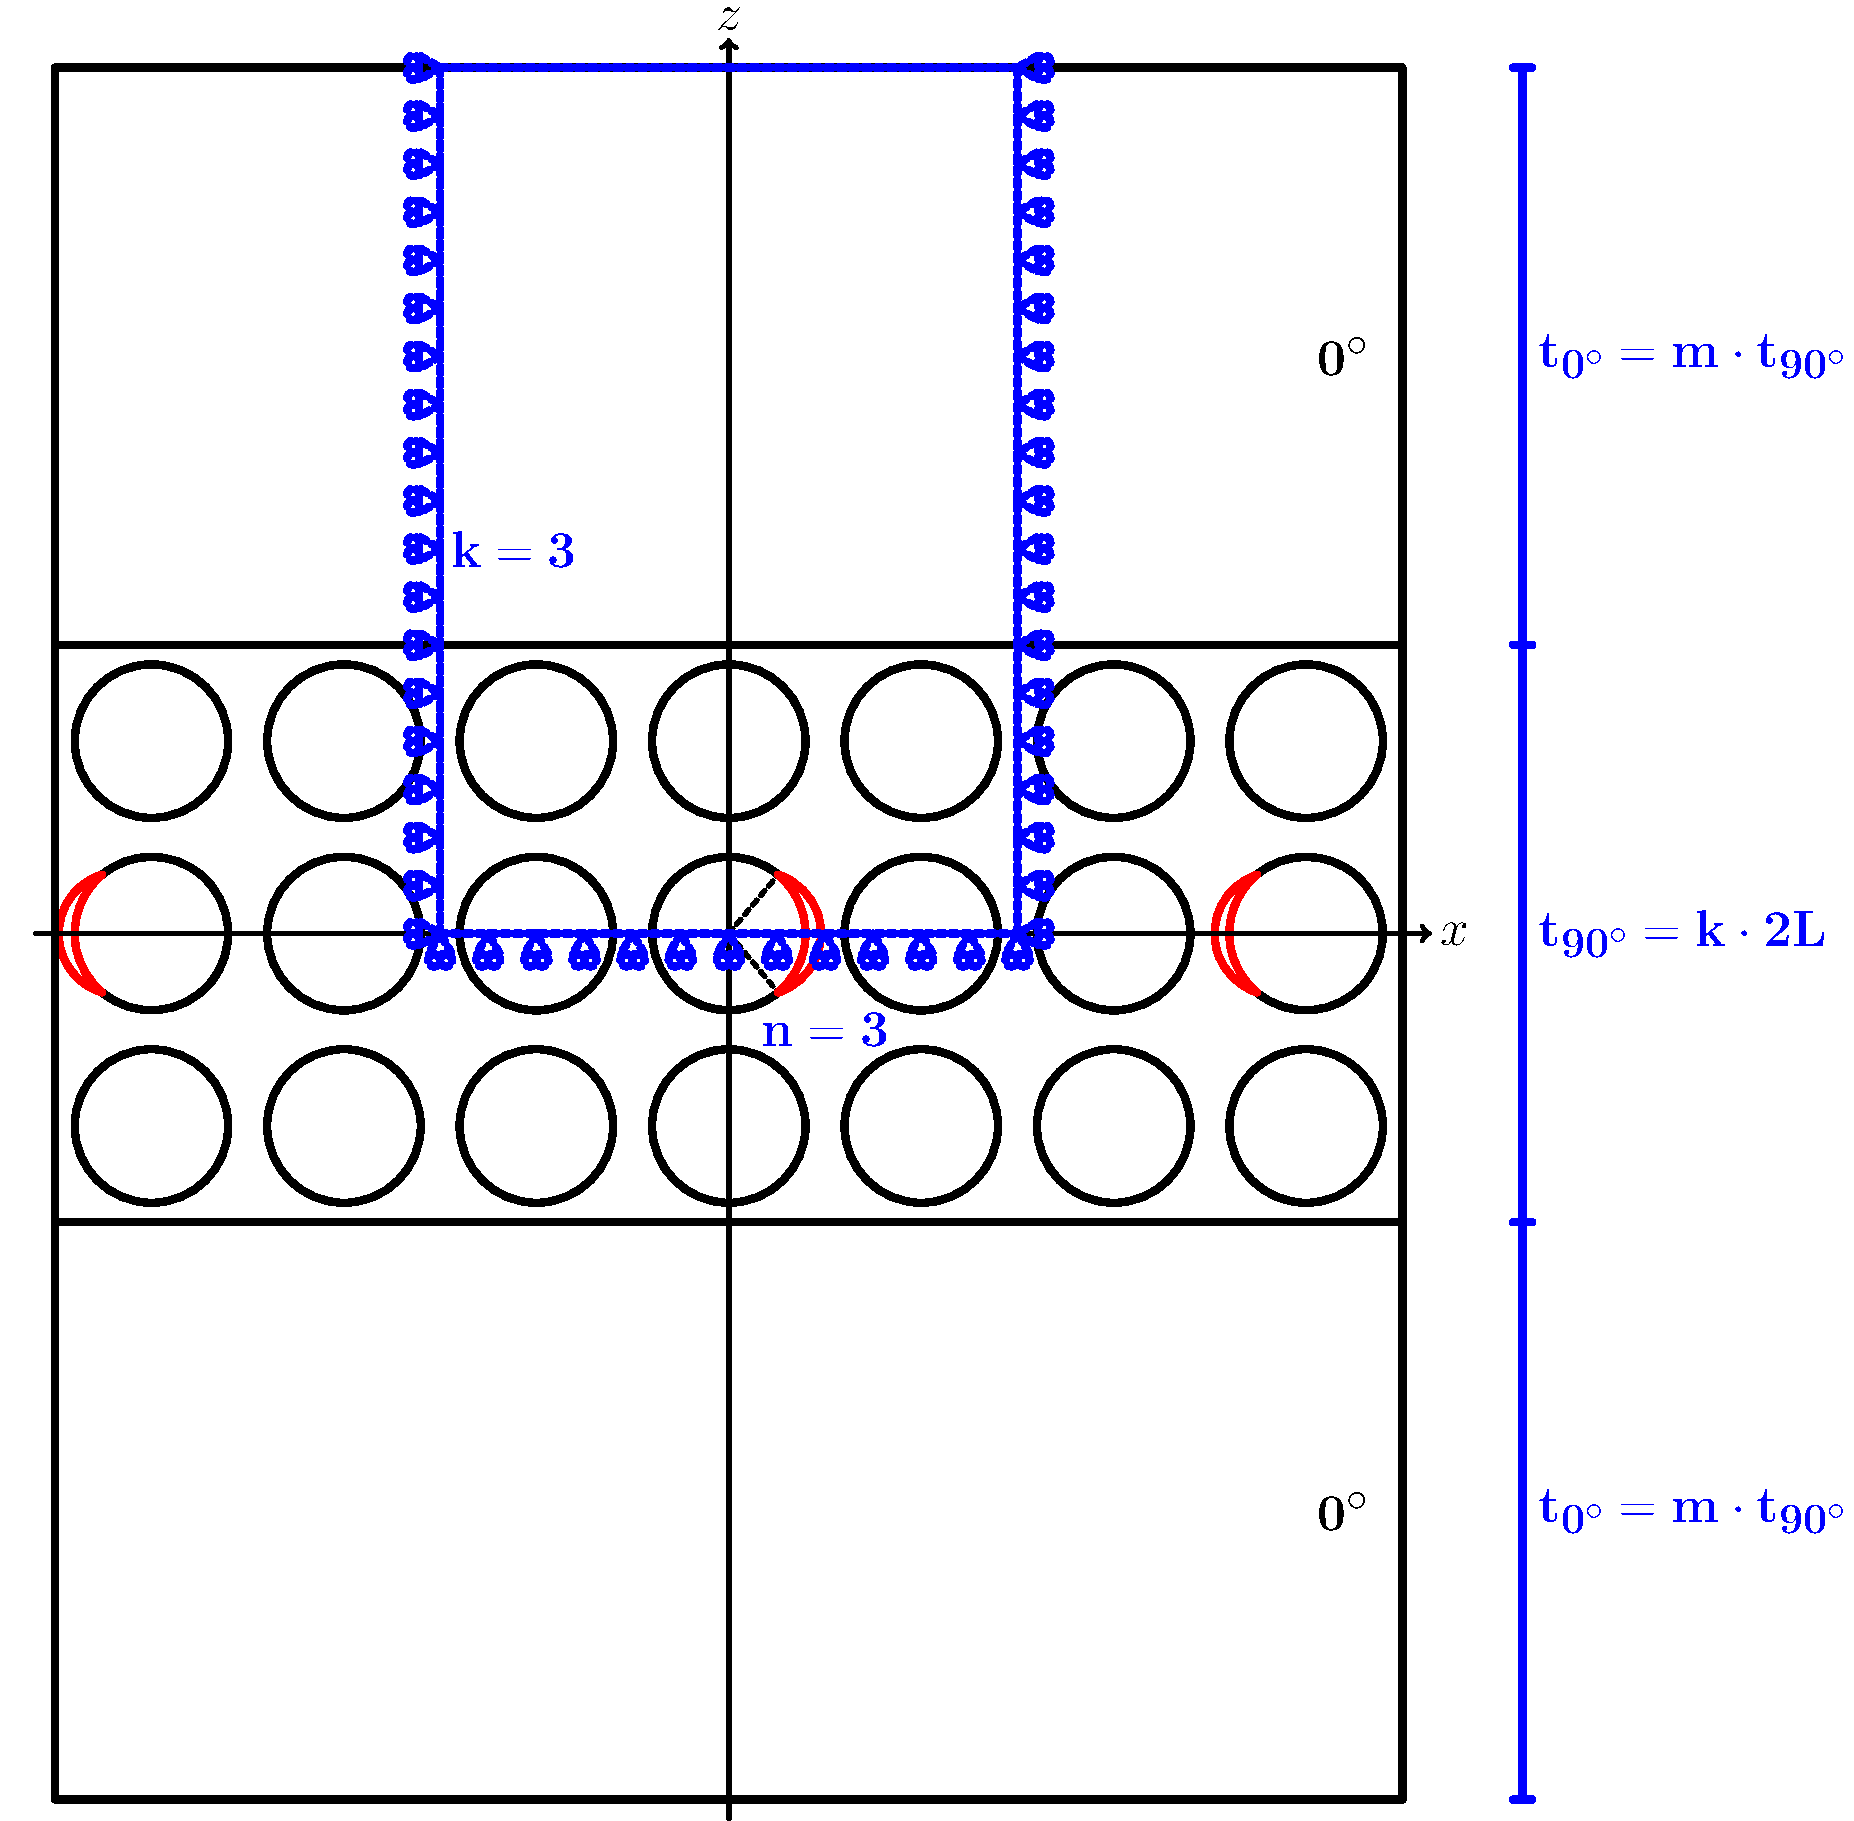
\includegraphics[width=0.9\textwidth]{paperC/ThickPly.pdf}
   %    \caption{Mutiple rows of fibers with a debond appearing every $n$ fibers within the central row: model $n\times k-free$ ($n=3$ and $k=3$ in the figure).}\label{paperC:subfig:thickply}
\caption{Models of $\left[0_{m\cdot k\cdot2L}^{\circ},90_{k\cdot2L}^{\circ},0_{m\cdot k\cdot2L}^{\circ}\right]$ laminates with a $90^{\circ}$ layer of variable thickness, determined by the number $k$ of ``rows'' of fibers along the vertical direction.  Debonds are repeating at different distances along the horizontal direction, measured in terms of the number $n-1$ of fully bonded fibers appearing between two consecutive debonds. $2L$ is the thickness of one-fiber row.}\label{chap3:paperC:fig:laminateModelsB}
\end{figure}

On top and below these $n\times k$ fibers, a homogenized $0^{\circ}$ ply is explicitly modelled, as shown in Figure~\ref{chap3:paperC:fig:laminateModelsB}. The thickness of these $0^{\circ}$ plies is defined as $m$ times the thickness $t_{90^{\circ}}$ of the central $90^{\circ}$ ply, where

\begin{equation}\label{chap3:paperC:eq:90thickness}
t_{90^{\circ}}=k2L.
\end{equation}

The RVE is symmetric with respect to the $x$-axis (horizontal axis), thus only half of it is explicitly modelled and conditions of symmetry are applied on the lower boundary of the RVE. On the left and right boundaries, conditions of coupling of the $x$-displacement (horizontal displacement) are applied, which implies that, as for the RVEs of paper A, the computed solution corresponds to the RVE repeating an infinite number of times to the left and to the right in a symmetric way with the respect to the side. Thus, the number $n$ of unit cells in the horizontal direction determines the distance between consecutive debonds in the horizontal direction, equal to $n-1$ fully bonded fibers. This family of RVEs is called $n\times k-m\cdot t_{90^{\circ}}$.\\
In order to understand the mechanisms influencing debond ERR by comparison with known conditions at the boundary, an additional family of RVEs is treated in which the $0^{\circ}$ layer is not present. In its place, different combinations of displacement boundary conditions are applied to the upper boundary. When the upper boundary is free, the $1\times 1-free$ RVE is defined, as in Paper A. The $1\times 1-coupling$ RVE is instead obtained when coupling of the vertical displacements $u_{z}$ is applied to the upper boundary (coupling condition). In the case a linear distribution of the horizontal displacement $u_{x}$ is applied to the upper boundary (H-condition), the RVE is refered to as $1\times 1-H$. Finally, when the linear distribution of the horizontal displacement $u_{x}$ is superimposed to the condition of coupling of the vertical displacements $u_{z}$ on the upper boundary, the $1\times 1-coupling+H$ RVE is obtained.\\
A constant $x$-strain equal to $1\%$ is applied to the left and right boundary. Contact between debond faces is considered frictionless. The fiber and matrix phases, respectively glass fiber and epoxy, are considered to be homogeneous, isotropic and linear elastic. The elastic properties of the $0^{\circ}$ ply are computed using Hashin's Concentric Cylinder Assembly model~\cite{Hashin1983} with the self-consistency scheme for the out-of-plane shear modulus of Christensen~\cite{Christensen1979}. The elastic properties of the three phases are reported in Table~\ref{chap3:paperC:tab:phaseprop}.

\begin{table}[!h]
 \centering
 \caption{Summary of mechanical properties of fiber, matrix and UD layer (GF: glass fiber; EP: epoxy; UD: glass-fiber/epoxy uni-directional properties).}%$E$ stands for Young's modulus, $\mu$ for shear modulus and $\nu$ for Poisson's ratio. Indexes $L$ and $T$ stand respectively for \emph{longitudinal} and \emph{transverse}.}
 \begin{tabular}{ccccccc}
\\
\small& \small\textbf{$V_{f}\left[\%\right]$}\  &\small \textbf{$E_{L}\left[GPa\right]$}\ & \small\textbf{$E_{T}\left[GPa\right]$}\  & \small\textbf{$G_{LT}\left[GPa\right]$} &\small\textbf{$\nu_{LT}\left[-\right]$} &\small \textbf{$\nu_{TT}\left[-\right]$} \\
\midrule
\small GF &\small-   &\small 70.0 &\small 70.0  &\small 29.2 &\small 0.2  &\small 0.2\\
\small EP    &-&\small 3.5 &\small 3.5   &\small 1.25 &\small  0.4&\small 0.4\\
\small UD&\small60.0&\small43.442&\small13.714&\small 4.315&\small 0.273&\small0.465\\
\end{tabular}
\label{chap3:paperC:tab:phaseprop}
\end{table}

The model is meshed with second order quadrilateral and triangular elements, while at the crack tip only second order quadrilateral elements are used with unitary aspect ratio, determined by the arc size $R_{f}\delta$ where $\delta$ is the angular size. The angular size $\delta$ of the elements at the crack tip is assumed as equal to $0.05^{\circ}$ based on the comparison with the Boundary Element Method (BEM) results provided in~\cite{Paris2007,Sandino2016} conducted in Paper A. Thus, the same level of accuracy of $5\%$ on ERR applies here.

\begin{figure}[!htb]
\centering
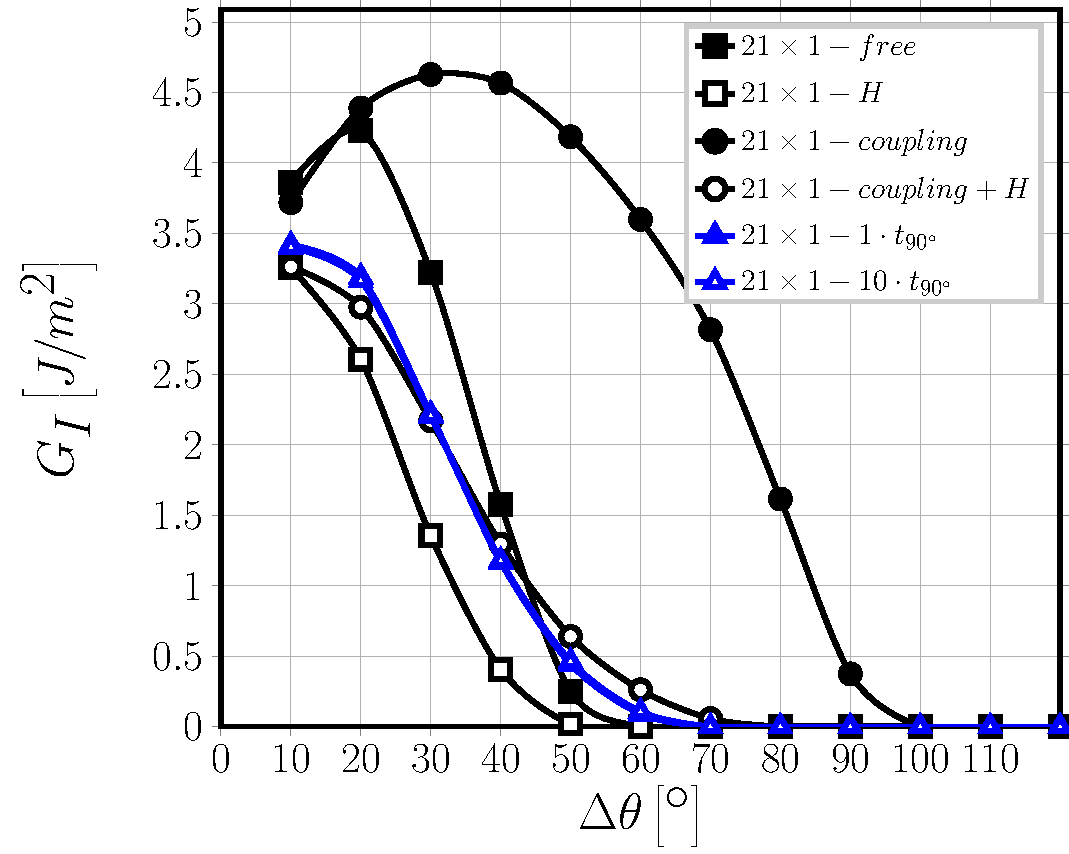
\includegraphics[width=0.9\textwidth]{paperC/nx1-1-vf60-GI.pdf}
\caption{Effect of the presence of the $0^{\circ}$ layer on Mode I ERR: models $21\times 1-free$, $21\times 1-H$, $21\times 1-coupling$, $21\times 1-coupling+H$, $21\times 1-1\cdot t_{90^{\circ}}$ and $21\times 1-10\cdot t_{90^{\circ}}$. $V_{f}=60\%$, $\bar{\varepsilon}_{x}=1\%$.}\label{chap3:paperC:fig:debonddebondGI}
\end{figure}

\begin{figure}[!htb]
\centering
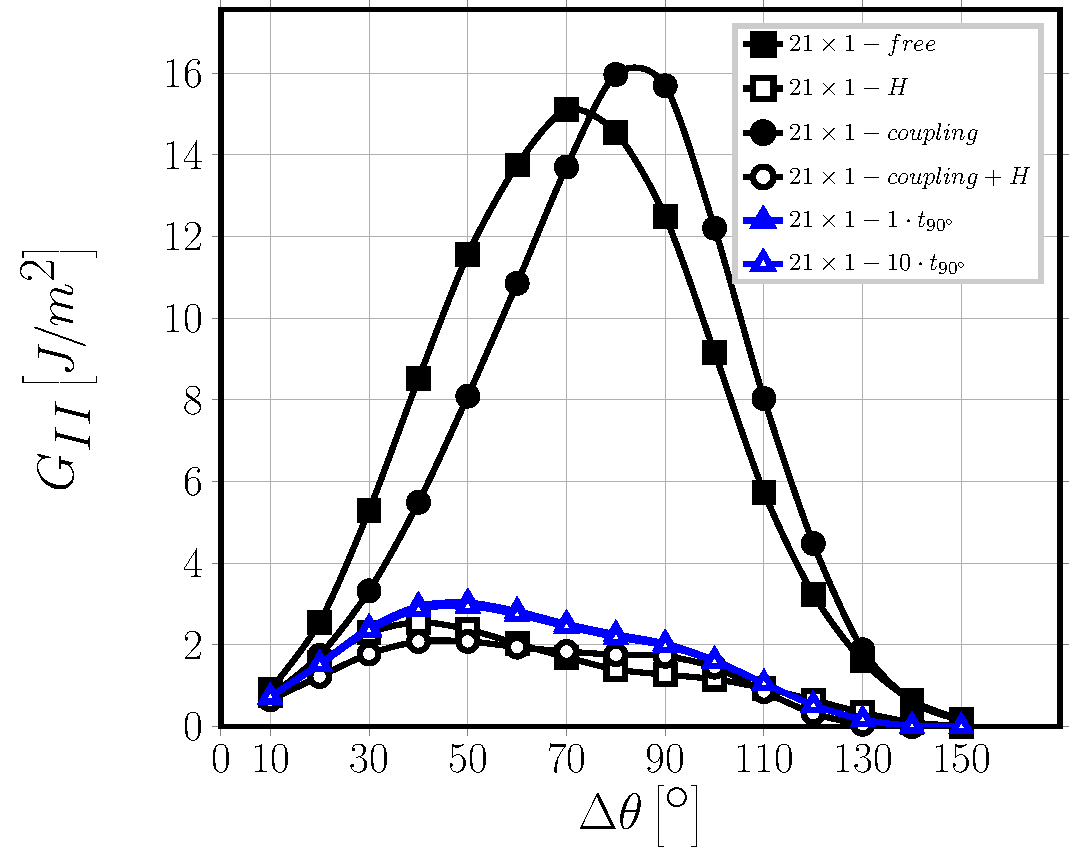
\includegraphics[width=0.9\textwidth]{paperC/nx1-1-vf60-GII.pdf}
\caption{Effect of the presence of the $0^{\circ}$ layer on Mode II ERR: models $21\times 1-free$, $21\times 1-H$, $21\times 1-coupling$, $21\times 1-coupling+H$, $21\times 1-1\cdot t_{90^{\circ}}$ and $21\times 1-10\cdot t_{90^{\circ}}$. $V_{f}=60\%$, $\bar{\varepsilon}_{x}=1\%$.}\label{chap3:paperC:fig:debonddebondGII}
\end{figure}

\begin{figure}[!htb]
\centering
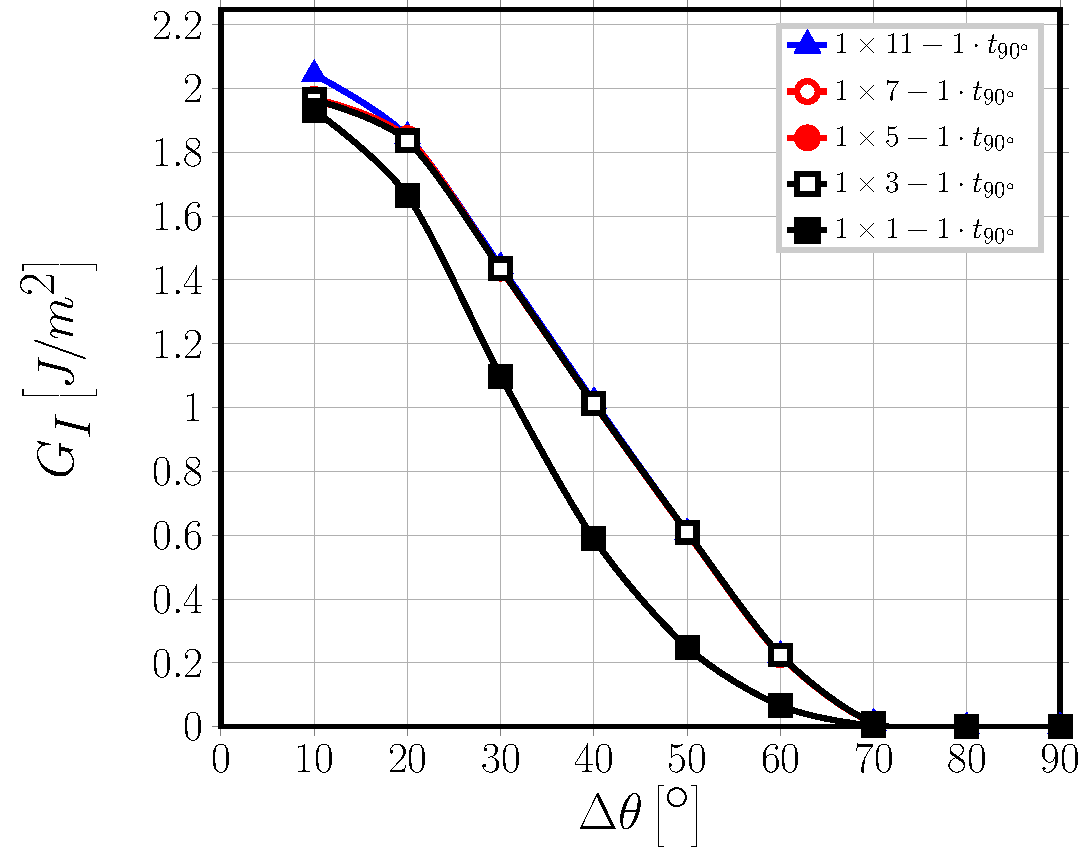
\includegraphics[width=0.9\textwidth]{paperC/1xk-1-vf60-GI.pdf}
\caption{Effect of the presence of undamaged fiber rows in the $90^{\circ}$ layer on debond-$0^{\circ}/90^{\circ}$ interface interaction for Mode I ERR: models $1\times k-1\cdot t_{90^{\circ}}$. $V_{f}=60\%$, $\bar{\varepsilon}_{x}=1\%$.}\label{chap3:paperC:fig:1kGI}
\end{figure}

\begin{figure}[!htb]
\centering
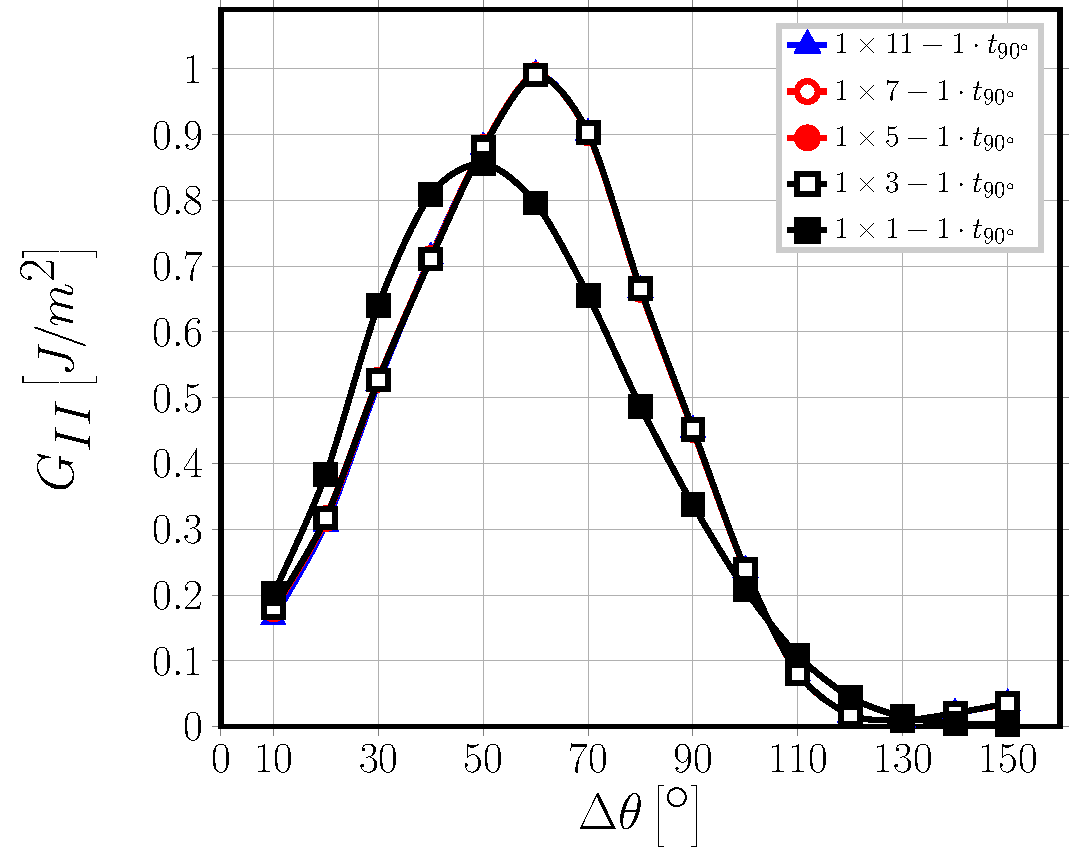
\includegraphics[width=0.9\textwidth]{paperC/1xk-1-vf60-GII.pdf}
\caption{Effect of the presence of undamaged fiber rows in the $90^{\circ}$ layer on debond-$0^{\circ}/90^{\circ}$ interface interaction for Mode II ERR: models $1\times k-1\cdot t_{90^{\circ}}$. $V_{f}=60\%$, $\bar{\varepsilon}_{x}=1\%$.}\label{chap3:paperC:fig:1kGII}
\end{figure}

The relevant results of Paper C are summarized in the following.

\begin{itemize}
\item Comparison between $n\times k-1\cdot t_{90^{\circ}}$ on one side and $n\times k-free$, $n\times k-H$, $n\times k-coupling$, $n\times k-coupling+H$ on the other (Figure~\ref{chap3:paperC:fig:debonddebondGI} and Figure~\ref{chap3:paperC:fig:debonddebondGII}) shows that the presence of the $0^{\circ}$ layer forces the $0^{\circ}/90^{\circ}$ interface to remain approximately straight and controls the uniformity of the horizontal displacement field in the composite, and thus in the $90^{\circ}$ ply. The presence of the $0^{\circ}$ layer thus causes a more homogeneous strain field, which reduces the Energy Release Rate at the debond tip.
\item Increasing the thickness of the $0^{\circ}$ layer, such that $\nicefrac{t_{0^{\circ}}}{t_{90^{\circ}}}$, does not lead to any significant change in debond ERR.
\item No effect of the $90^{\circ}$ layer thickness, measured in terms of number $k$ of fiber rows, is observed, as shown in Figure~\ref{chap3:paperC:fig:1kGI} and Figure~\ref{chap3:paperC:fig:1kGII}. Only if the thickness is reduced to only one fiber row, the Energy Release Rate decreases in value.
\item These results strengthen the claim that the ply-thickness effect does not influence the growth of individual debonds, as observed previously in the literature~\cite{Saito2012,Herraez2015,Velasco2018, Paris2018}.
\end{itemize}

%%%%%%%%%%%%%%%%%%%%%%%%%%%%%%%%%%%%%%%%%%%%%%%%%%%%%%%%%%%%%%%%%%%%%%%
%      Paper D
%%%%%%%%%%%%%%%%%%%%%%%%%%%%%%%%%%%%%%%%%%%%%%%%%%%%%%%%%%%%%%%%%%%%%%%
\section{Paper D}
\section*{Growth of interface cracks on consecutive fibers: on the same or on the opposite sides?}

In Paper D, fiber/matrix interface crack growth is studied in Representative Volume Elements of thick UD composites subjected to transverse tensile loading. Similarly to PAper A and Paper B, the unit cell of one fiber and its surrounding matrix, shown in Figure~\ref{chap3:paperB:fig:modelschem}, represents the basic element of the RVE. The unit cell has a size of $2L\times2L$, where

\begin{equation}\label{chap3:paperC:eq:LVf}
L=\frac{R_{f}}{2}\sqrt{\frac{\pi}{V_{f}}},
\end{equation}

$R_{f}$ is the fiber radius, assumed again to be equal to $1\ \mu m$, and $V_{f}$ is the fiber volume fraction.\\
The RVE is formed by $n$ unit cells in the horizontal (loading) direction and $k$ unit cells in the vertical (through-the-thickness) direction (see Figure~\ref{chap3:paperD:fig:coupling-rve} and Figure~\ref{chap3:paperD:fig:asymm-rve}). The fiber of the unit cell placed in the center of the RVE is always partially debonded, and the debond has an angular size $\Delta\theta$ which can vary between $10^{\circ}$ and $150^{\circ}$.

\begin{figure}[!htb]
\centering
  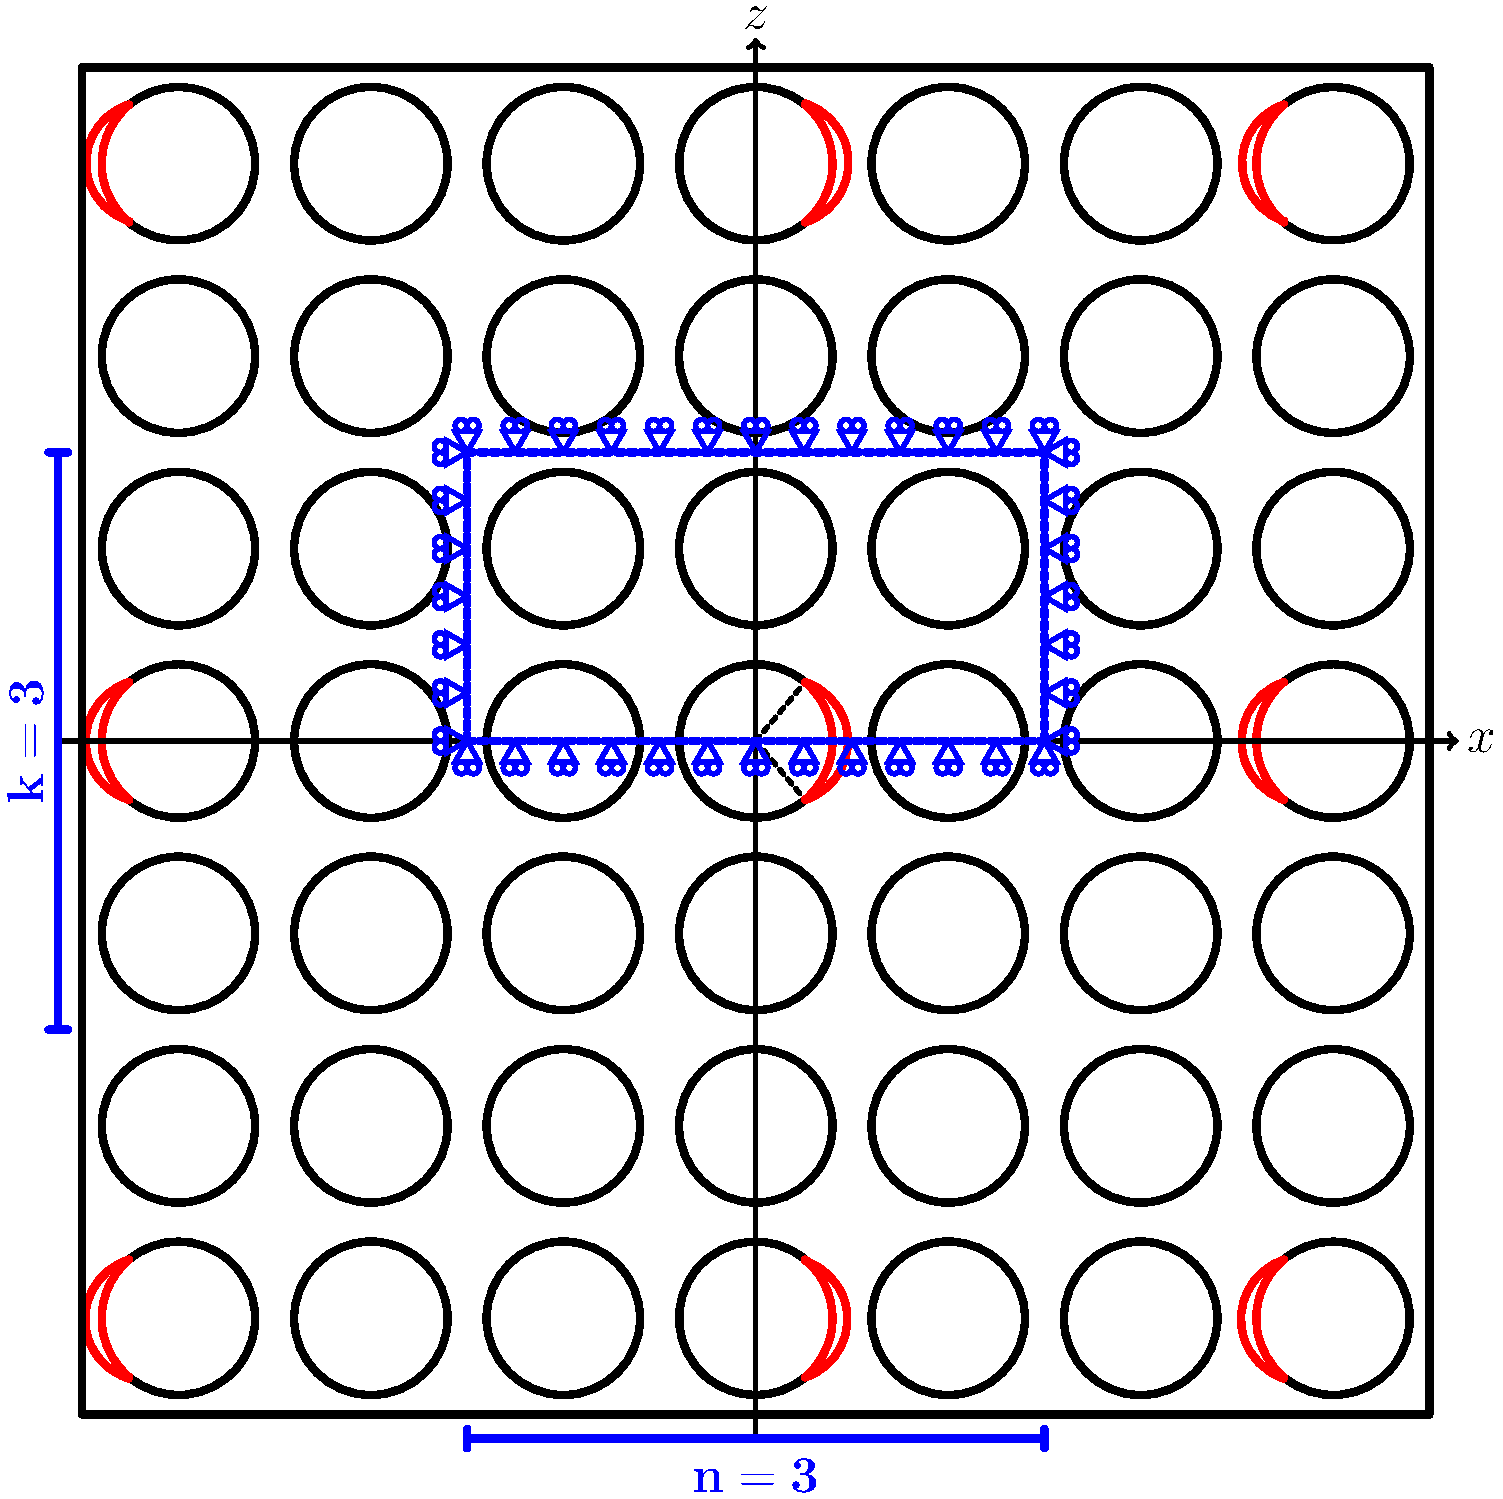
\includegraphics[width=0.9\textwidth]{paperD/coupling.pdf}
\caption{Representative Volume Element $n \times k-symm$ of a UD composite with debonds appearing after $n-1$ and after $k-1$ undamaged fibers respectively in the horizontal and vertical direction. In the vertical direction, on fibers belonging to the same ´´column", debonds are located always on the same side.}\label{chap3:paperD:fig:coupling-rve}
\end{figure}

The RVE is symmetric with respect to the $x$-axis (horizontal axis), thus only half of it is explicitly modelled and conditions of symmetry are applied on the lower boundary of the RVE. On the left and right boundaries, conditions of coupling of the $x$-displacement (horizontal displacement) are applied, which implies that, as for the RVEs of Paper A and Paper B, the computed solution corresponds to the RVE repeating an infinite number of times to the left and to the right in a symmetric way with the respect to the side. Thus, the number $n$ of unit cells in the horizontal direction determines the distance between consecutive debonds in the horizontal direction, equal to $n-1$ fully bonded fibers. On the top boundary, two different sets of boundary conditions are applied. The first are conditions of coupling of the vertical displacement $u_{z}$, expressed as

\begin{equation}
u_{z}\left(x,h\right)=u_{z}^{\nu},
\end{equation}

where $h=kL$ corresponds to the height of the RVE and $u_{z}^{\nu}$ represents the unknown constant vertical displacement of the upper boundary due to Poisson's effect, which is calculated as part of the elastic solution. This set of conditions implies that the computed solution is that of the RVE repeating an infinite number of times in the vertical direction in a symmetric way as shown in Figure~\ref{chap3:paperD:fig:coupling-rve}, i.e. if the debond in the central unit cell appears on the right, all the debonds in the vertical direction aligned with it will be placed on the right half of their respective fiber. This family of RVEs is referred to as $n\times k-symm$.

\begin{figure}[!htb]
\centering
  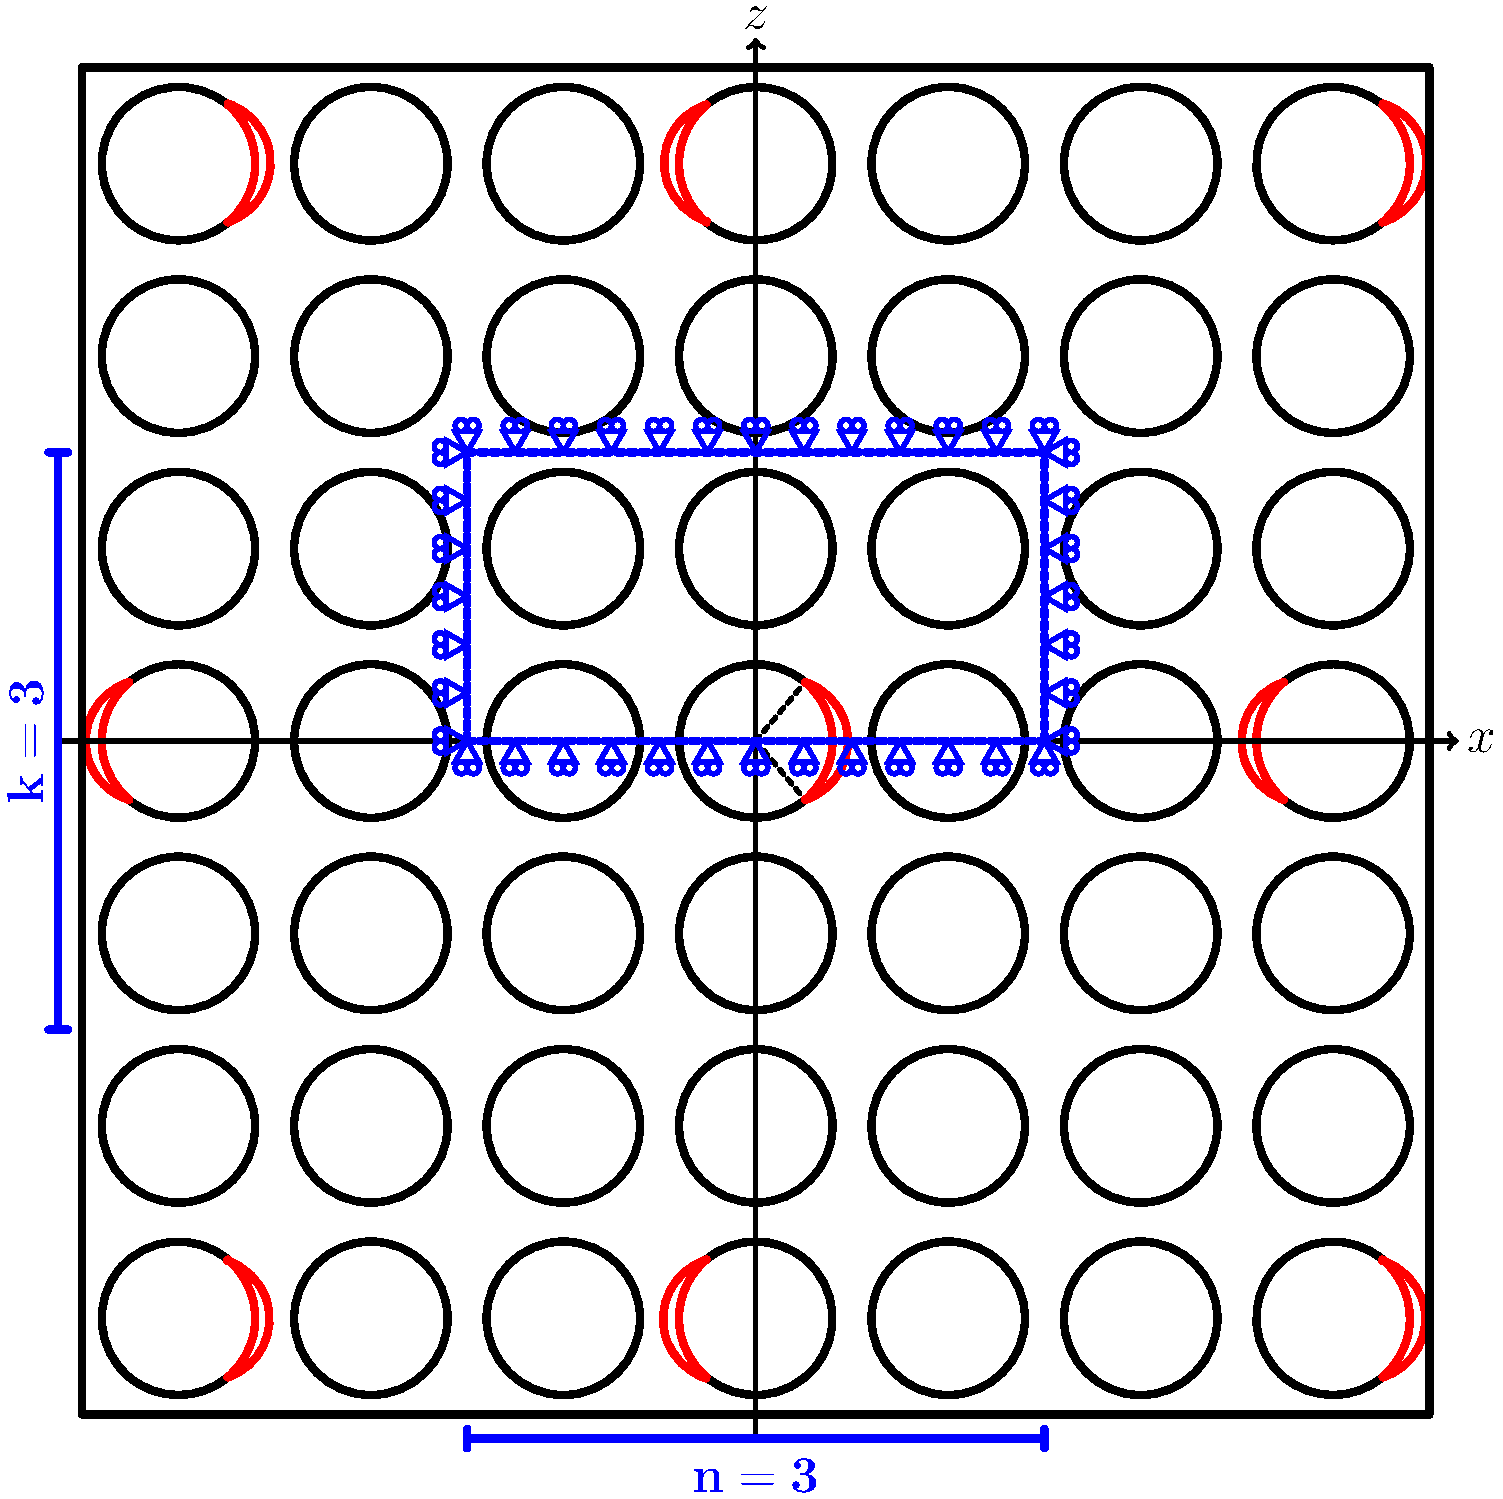
\includegraphics[width=0.9\textwidth]{paperD/asymm.pdf}
\caption{Representative Volume Element $n \times k-asymm$ of a UD composite with debonds appearing after $n-1$ and after $k-1$ undamaged fibers respectively in the horizontal and vertical direction. In the vertical direction, on fibers belonging to the same ´´column", debonds are located on the opposite sides of consecutive fibers.}\label{chap3:paperD:fig:asymm-rve}
\end{figure}

The second set of conditions represents instead anti-symmetric coupling conditions, expressed as

\begin{equation}
u_{z}\left(x,h\right)-u_{z}\left(0,h\right)=-\left(u_{z}\left(-x,h\right)-u_{z}\left(0,h\right)\right),
\end{equation}

\begin{equation}
u_{x}\left(x,h\right)=-u_{x}\left(-x,h\right),
\end{equation}

where $h$ represents the height of the RVE and $u_{z}\left(0,h\right)$ stands for the unknown vertical displacement of the upper boundary's mid-point caused by Poisson's effect, which is evaluated as part of the elastic solution. Similarly to $n\times k-symm$, this set of conditions implies that the RVE is repeating infinite times in the vertical direction. However, the unit cell is repeated anti-symmetrically this time: if a debond is placed on the right side of its fiber, the next one aligned in the vertical direction will appear on the left side (Figure~\ref{chap3:paperD:fig:asymm-rve}). This second set of RVEs is named $n\times k-asymm$.\\
A constant horizontal strain ($x$-strain) equal to $1\%$ is applied to the left and right boundary. Frictionless contact is considered between debond faces. The fiber and matrix phases, respectively glass fiber and epoxy, are considered to be homogeneous, isotropic and linear elastic. The elastic properties of the two phases are reported in Table~\ref{chap3:paperC:tab:phaseprop}.

\begin{table}[!h]
 \centering
 \caption{Material properties of glass fiber and epoxy adopted in the present study.}
 \begin{tabular}{cccc}
\\
\textbf{Material} & \textbf{$E\left[GPa\right]$}\ & \textbf{$\mu\left[GPa\right]$} & \textbf{$\nu\left[-\right]$} \\
\midrule
Glass fiber    & 70.0  & 29.2   & 0.2  \\
Epoxy    & 3.5    & 1.25   & 0.4
\end{tabular}
\label{chap3:paperD:tab:phaseprop}
\end{table}

The model is meshed with second order quadrilateral and triangular elements, while at the crack tip only second order quadrilateral elements are used with unitary aspect ratio, determined by the arc size $R_{f}\delta$ where $\delta$ is the angular size. The angular size $\delta$ of the elements at the crack tip is assumed as equal to $0.05^{\circ}$ based on the comparison with the Boundary Element Method (BEM) results provided in~\cite{Paris2007,Sandino2016} conducted in Paper A. Thus, the same level of accuracy of $5\%$ on ERR applies here.

%%%%%%%%%%%%%%%%%%%%%%%%%%%%%%%%%%%%%%%%%%%%%%%%%%%%%%%%%%%%%%%%%%%%%%%
%      Paper E
%%%%%%%%%%%%%%%%%%%%%%%%%%%%%%%%%%%%%%%%%%%%%%%%%%%%%%%%%%%%%%%%%%%%%%%
\section{Paper E}
\section*{Estimating the average size of fiber/matrix interface cracks in ud and cross-ply laminates}
